% !TEX TS-program = xelatex

\chapter{Geometric models}
\label{chapt:4}

Julia |Plasm| is the best choice to write symbolic geometric models for Building Information Modeling (BIM) and Computer-Aided Design (CAD).  Geometric models specify the physical appearance of Architecture, Engineering, and Construction products at any scale, from structural and envelope components to whole buildings and built environments, and are used for design, tender, contract, and collaboration. We ported the  functional language |Plasm| to Julia for better supporting design, model generation, and visualization of geometric objects.
In this chapter we introduce the great expressive power of |Plasm| geometric types and parametric functions, as well the simple methods used to build parametric assemblies, where objects itself can be used as actual parameters. We show also that |Plasm| offers a  general mechanism (Julia dictionaries) to export models characterized by colors, textures, materials, and so on. |Plasm| can be even embedded in the |Juπpiter| platform in order to document the design choices step-by-step in digital notebooks.

\section{Plasm geometric types}\label{sect:4-1}

Even if Julia does not pretend the user specifies the type of data objects, which are inferred at compile time, it may always be useful to annotate with their type the parameters and the returned value from function applications in order to get faster codes from the Julia compiler. The best reason concerns program documentation, making it easier to understand the Julia's sources.

Let's remember that |Plasm| derives from three founts: (1) the |PLaSM| classic set up on |FL| functional combinators; (2) the porting to Python (object-oriented language), and finally (3) the embedding into Julia (functional and multi-paradigm), after several years of algebraic research finalized to understand the role of topology in elaborating digital  geometric models. 

This development defined different data types and user structures, which the current version of the language proudly unifies by scheduling them to different roles and uses.
 

\begin{enumerate}
\item 
The Hierarchical Polyhedral Complex, now denoted in Julia |Plasm| as the |Hpc| datatype, was characterized by models defined as aggregation of multidimensional convex cells, described only by their vertices and by multidimensional affine matrices.

\item 
Our research about algebraic topology of geometric design directed us to design the Linear Algebraic Representation, currently the |Lar| datatype, used to work with chain complexes, and able to  fully specify the geometry and topology of the \emph{solid objects} under consideration, even non-manifold.

\item 
Finally, a third Julia’s user-defined |struct|, named |Geo| for Geometry, is being used as container of huge datasets for |Plasm|-coded generation of |BIM| objects and 3D point clouds from surveys.  
\end{enumerate}


\subsection*{Hpc Type}\label{sect:4-1-1}

This recursive type is mainly used for geometric object definition, including the hierarchical values generated by the |STRUCT| function, and interactive graphics visualization on the display device.

An object of |Hpc| type has three fields: a multidimensional matrix |T::MatrixNd|; a vector |childs| (i.e., children) either of elements |Hpc| or of elements |Geometry|, and a |Properties| field of dictionary type, i.e., |Dict{Any, Any}|.

The |mutable struct Hpc| is a typical recursive data structure to represent dynamically a data object of tree type, where the | children | nodes of a node may be in any number since stored into a Julia’s |Vector|.

\begin{lstlisting}[language=JuliaLocal, style=julia, mathescape = true] 
mutable struct Hpc
T::MatrixNd
childs::Union{Vector{Hpc}, Vector{Geometry}}
properties::Dict{Any, Any}
# constructor
   function Hpc(T::MatrixNd=MatrixNd(0), childs:: Union{Vector{Hpc}, Vector{Geometry}}=[], properties=Dict())
      self = new()
      self.childs = childs
      self.properties = properties
      if length(childs) ) 0
         Tdim = maximum([dim(child) for child in childs]) + 1
         self.T = embed(T, Tdim)
      else
         self.T = T
      end
      return self
   end
end
\end{lstlisting}



\subsection*{Lar Type}\label{sect:4-1-2}

The |mutable struct Lar| is used to represent synthetically a generic cellular or chain complex, together with some of its properties. Given |obj::Lar|, it represents with |obj.d|, |obj.m|, |obj.n|, |obj.V|, and |obj.C|, respectively, the intrinsic dimension (1 for curves, 2 for surfaces, 3 for solids), the number of its coordinates, the number of vertices, and a dictionary of of chain bases or chain operators, stored when already available throughout a computation.

\begin{lstlisting}[language=JuliaLocal, style=julia, mathescape = true] 
mutable struct Lar
   d::Int # intrinsic dimension
   m::Int # embedding dimension (rows of V)
   n::Int # number of vertices  (columns of V)
   V::Matrix{Float64} # object geometry
   C::Dict{Symbol, AbstractArray} # object topology (C for cells) 
   # inner constructors
   Lar() = new( -1, 0, 0, Matrix{Float64}(undef,0,0), Dict{Symbol, AbstractArray}() )
   Lar(m::Int,n::Int) = new( m,m,n, Matrix(undef,m,n), Dict{Symbol,AbstractArray}() )
   Lar(d::Int,m::Int,n::Int) = new( d,m,n, Matrix(undef,m,n), Dict{Symbol,AbstractArray}() ) 
   Lar(V::Matrix) = begin m, n = size(V); new( m,m,n, V, Dict{Symbol,AbstractArray}() ) end
   Lar(V::Matrix,C::Dict) = begin m,n = size(V); new( m,m,n, V, C )  end
   Lar(d::Int,V::Matrix,C::Dict) = begin m,n = size(V); new( d,m,n, V, C )  end
   Lar(d,m,n, V,C) = new( d,m,n, V,C )
end
\end{lstlisting}



\subsection*{Geo type}\label{sect:4-1-3}

A |mutable struct Geometry| is used as a container for single whole geometric objects, allowing to store the various dimensional cellular subcomplexes that partition the geometric value. Conversely, any hierarchical assembly is stored in |Plasm| within a mixture of |Hpc| and |Geometry| nodes. The |Geometry| data structure contains arrays of integers, denoting the ordered bases of the topological chains of different dimensions that decompose the represented geometric value. It also contains a numeric |db| (data base), implemented as a Julia dictionary with key the (suitably rounded) coordinate vector sof vertex |point| and with value the corresponding integer index.

\begin{lstlisting}[language=JuliaLocal, style=julia, mathescape = true] 
mutable struct Geometry
   db::Dict{Vector{Float64}, Int}
   points::Vector{Vector{Float64}}
   edges::Vector{Vector{Int}}
   faces::Vector{Vector{Int}}
   hulls::Vector{Vector{Int}}
   # constructor
   function Geometry()
   self = new(
      Dict{Vector{Float64}, Int}(),
      Vector{Vector{Float64}}(),
      Vector{Vector{Int}}(),
      Vector{Vector{Int}}(),
      Vector{Vector{Int}}(),
   )
   return self
   end
end
\end{lstlisting}


\subsection*{Topological types}\label{sect:4-1-4}

Some abstract types are defined in |Plasm| in order to characterize and document the type of variables and/or parameters within complicated definitions and function codes. They are mainly used within the structures of |Lar| type, to document the topology, and are defined as global |const| symbols.

\begin{lstlisting}[language=JuliaLocal, style=julia, mathescape = true] 
const Points = Matrix{number}
const Cells = Vector{Vector{Int}}
const Cell = SparseVector{Int8, Int}
const Chain = SparseVector{Int8,Int}
const ChainOp = SparseMatrixCSC{Int8,Int}
const ChainComplex = Vector{ChainOp}
\end{lstlisting}

The |Cells| type stores the cellular bases and some subsets of cells as |Vector| of |Vector| of integers. The |Cell| type is utilized to memorize a single cell's (sparse)  representation. The |Chain| type item equals the cell type, and is used only for documentation aims. The |ChainOp| type allows the storage of the topological operators, including boundary and coboundary, and other higher degree operators, e.g., |FV|. The |ChainComplex| type is employed as the multidimensional |Vector| store of chain complexes, by now only in 2D and 3D, with two and three |ChainOp| sparse matrices, respectively.

\begin{coding}[3-cube topology is a ChainOp object]\
The expression |cube.C[:FV]| returns a dictionary value of type |Cells|, which contains the basis of our cubic cellular complex.  |KFV| is of type |ChainOp|:

\begin{lstlisting}[language=JuliaLocal, style=julia, mathescape = true] 
cube = LAR(CUBE(3))			#=
Lar(3, 3, 8, [3.0 0.0 … 3.0 0.0; 3.0 3.0 … 3.0 3.0; 0.0 0.0 … 3.0 3.0], Dict{Symbol, AbstractArray}(:CV =) [[1, 2, 3, 4, 5, 6, 7, 8]], :FV =) [[1, 2, 3, 4], [3, 4, 5, 6], [1, 3, 5, 7], [2, 4, 6, 8], [1, 2, 7, 8], [5, 6, 7, 8]], :EV =) [[3, 4], [2, 4], [1, 2], [1, 3], [5, 6], [4, 6], [3, 5], [5, 7], [1, 7], [6, 8], [2, 8], [7, 8]])) =#

FV = cube.C[:FV]			#=
6-element Vector{Vector{Int64}}:
 [1, 2, 3, 4]
 [3, 4, 5, 6]
 [1, 3, 5, 7]
 [2, 4, 6, 8]
 [1, 2, 7, 8]
 [5, 6, 7, 8]			=#

KFV = lar2cop(FV::Cells)::ChainOp		#=
6×8 SparseArrays.SparseMatrixCSC{Int8, Int64} with 24 stored entries:
 1  1  1  1  ⋅  ⋅  ⋅  ⋅
 ⋅  ⋅  1  1  1  1  ⋅  ⋅
 1  ⋅  1  ⋅  1  ⋅  1  ⋅
 ⋅  1  ⋅  1  ⋅  1  ⋅  1
 1  1  ⋅  ⋅  ⋅  ⋅  1  1
 ⋅  ⋅  ⋅  ⋅  1  1  1  1			=#
\end{lstlisting}
Of course, |(typeof(FV)==Cells) && (typeof(KFV)==ChainOp) # =) true|, 
since |lar2cop| : Cells $\to$ |ChainOp|.
\end{coding}

\begin{remark}[About sparsity]
While in this small case, the |KFV| matrix is not very sparse, the sparsity overgrows as the cellular complex proliferates, since the non-zero elements grow linearly with the number of cells. In contrast, the zero elements grow quadratically (with the matrix dimension).
\end{remark}
\begin{remark}[Global view of incidencies]
See, by inspection of |KFV|, that each face is incident to 4 cube vertices and each vertex is incident to 3 faces.
\end{remark}


\section{Plasm parametric primitives}\label{sect:4-2}

In this section, we introduce and exemplify several features of |Plasm| working with geometric objects. The |Plasm| package is quite different from most geometric and graphics |API|s since it is based on |FL|-style combinators.


\subsection{Geometric Transformations}\label{sect:4-2-1}

The user interface to affine coordinate transformation of geometric objects is given through standard Julia functions and matrices. Internally, |Plasm| implements such mapping of local coordinates using its own multidimensional matrix type, called |MatrixNd|, and the use of the field |T::MatrixNd| within the recursive datatype |Hpc|.

\begin{definition}[Geometric transformation]
A \emph{geometric transformation} is a bijective function, i.e., a one-to-one (injective) and onto (surjective) mapping $\mathbb{E}^d \to \mathbb{E}^d$. 
\end{definition}

By definition, geometric transformations of plane or space are invertible, and hence represented by invertible square matrices. We will see that \emph{rotation}, \emph{scaling}, and \emph{shearing} are linear transformations; \emph{translation} is affine. 


\subsubsection*{Homogeneous Coordinates}

In computer graphics the \emph{homogeneous coordinates} are often used instead of Cartesian coordinates. In the homogeneous plane or space, lines are mapped to lines, but parallel lines are not conserved parallel. The main reason for this change is the ability to treat affine maps (translation) as linear, and combine smoothly with linear maps (rotation, scaling, etc.)

In homogeneous coordinates the Euclidean plane $\mathbb{E}^2 \,\backslash\, \{\v{0}\}$ is considered in bijective correspondence with the bundle of lines in $\mathbb{E}^3 \,\backslash\, \mathbb{E}^2$ (a model for the projective plane) so that each point $(x,y)\in\E^2$ corresponds to a line $\lambda(W, X, Y)$ such that $(x, y) \equiv \frac{W}{W}, \frac{X}{W}, \frac{Y}{W}) = (1, x, y)$. Same for each $\E^d$, $d \geq 2$. After the division, homogeneous coordinates are said \emph{normalized}.

\begin{figure}[htbp] %  figure placement: here, top, bottom, or page
   \sidecaption[t]
   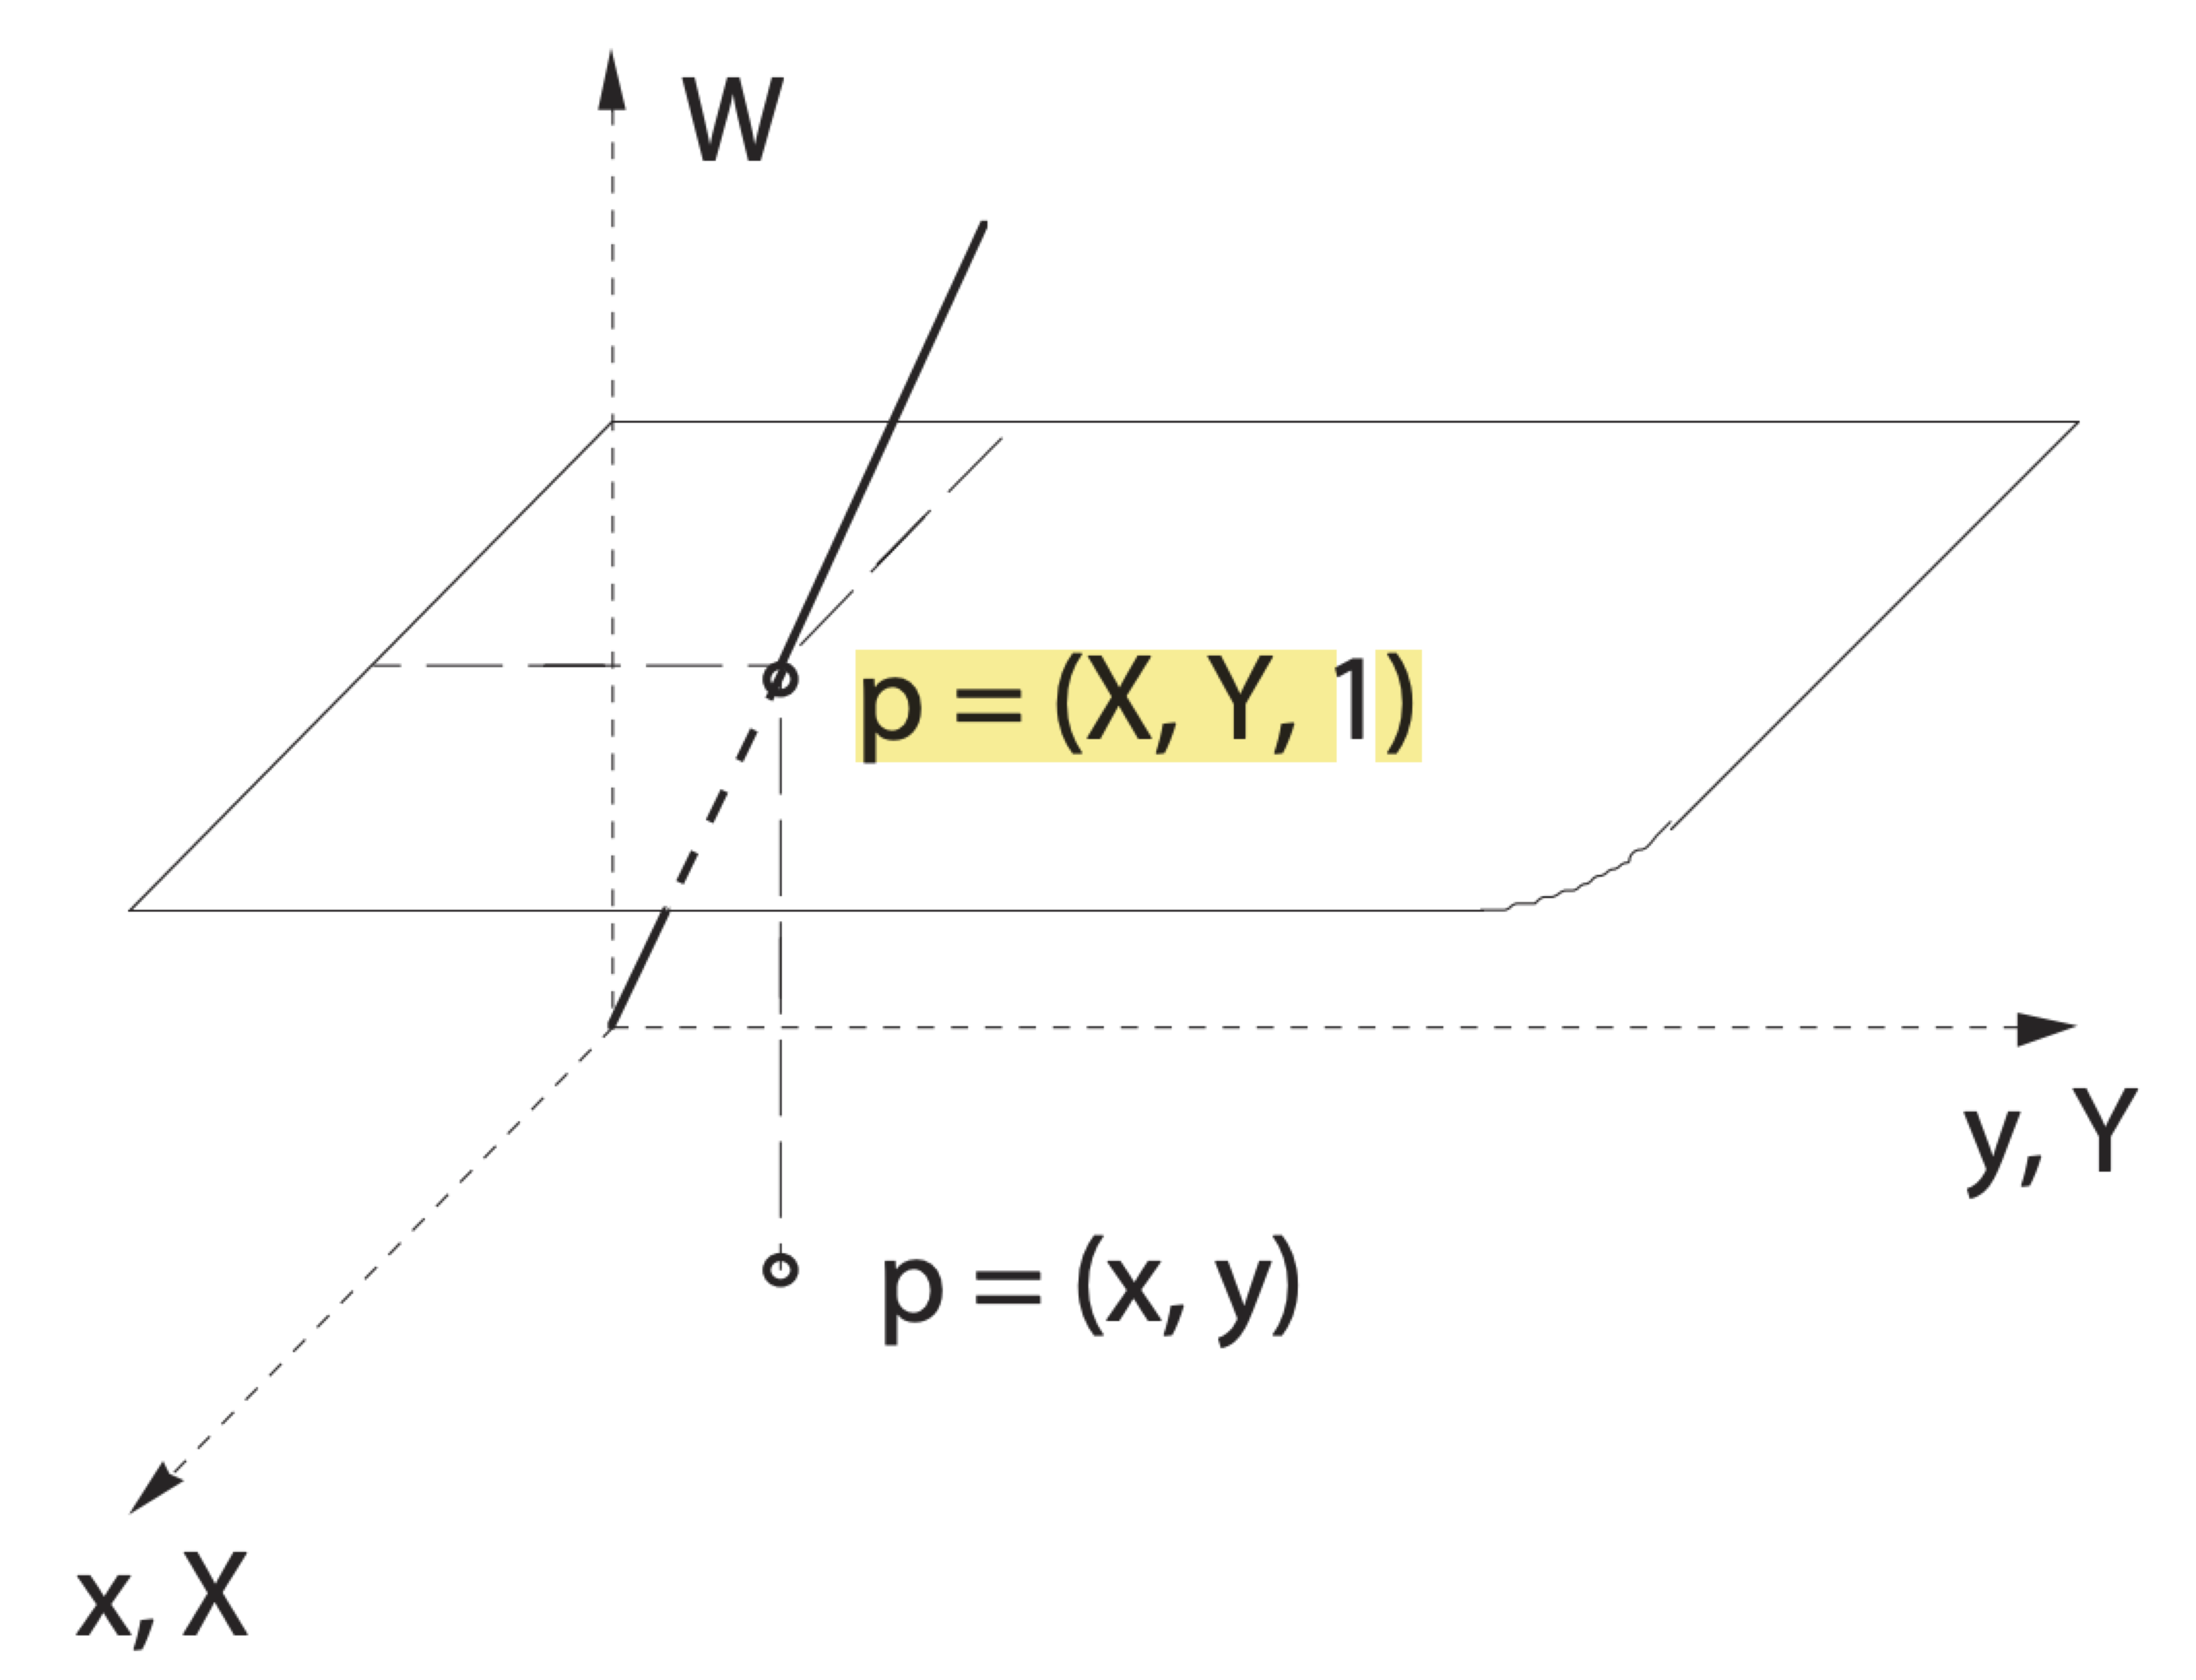
\includegraphics[width=2in]{chapter-04/figs/homog-2d} 
   \caption{The homogeneous plane is a model of a projective plane, where all finite points have a homogeneous coordinate equal to one, and the points at infinity have it equal to zero. All the points at infinity form the line at infinity, and all the lines at infinity form the plane at infinity.}
   \label{fig:example}
\end{figure}

In |Plasm|, by design choice to make the multidimensional approach to geometric design more accessible, the added homogeneous coordinate is the first, not the last, as we may see in many computer graphics books.

Even more, for the sake of clarity, we can use the |HOMO| operator to transform a $d\times d$ matrix in a $(d+1)\times(d+1)$ matrix, i.e., a $3\times 3$ on the 2D plane and $4\times 4$ on 3D space. The type of returned matrix is |MatrixNd|, which is used for dimension-independent programming.

Homogeneous coordinates allow to combine linearly all transformations, using products of their matrices in homogeneous coordinates. In the remainder of this section we describe the geometric effect of each transformation and the structure of the corresponding matrices. 

\begin{remark}The reader should note that our maps or transformations are invertible functions of a space into itself (automorphisms), represented (even translation, as we will see) by square matrices, i.e. are \emph{rank 2} tensors. Since they are also |Plasm| functions, can be \emph{applied} to geometric objects; as matrices, they multiply the object coordinates.
\end{remark}




\subsection*{2D rotation}\label{sect:4-2-1}

In a \emph{planar rotation} all points of the 2D plane move along an arc of circle, with same angle at center, while the center is the only fixed point. In  a \emph{space rotation} there is a straight line of fixed points (the axis) passing for the origin. All the other 3D points describe a circle arc with the same angle along the plane (orthogonal to rotation axis) which they belong to. 

Let us show (see Figure~\ref{fig:rotmatrix}) how unit vectors $\v{e}_1 = \vet{1 \\ 0}$ and $\v{e}_2 = \vet{0 \\ 1}$, columns of the matrix $\mat{\v{e}_1 & \v{e}_2 } $ are transformed by the (yet unknown) $\T{R}(\alpha)$ rotation matrix into the columns of the matrix at right-hand side:
\[
\mat{\cos\alpha & -\sin\alpha\\ \sin\alpha & \cos\alpha}
=
\T{R}(\alpha)\,\mat{\v{e}_1 & \v{e}_2 }. 
\quad
\mbox{Hence we have:}
\quad
\T{R}(\alpha) = \mat{\cos\alpha & -\sin\alpha\\ \sin\alpha & \cos\alpha}
\]


There is only one class of planar rotations, parameterized by $\alpha$, the \emph{rotation angle} about the origin. Conversely, we will see three classes of elementary space rotations, parameterized by $\alpha_x, \alpha_y, \alpha_z$, the rotation angles about each coordinate axis.


\begin{coding}[Plasm notation for rotation]
The plane rotation function in |Plasm| is: |R([1,2])($\alpha$)| because its effect is to change the first and second coordinates of the 2D model it is applied to. They are applied to a planar geometric object of |Hpc| type, by using the |STRUCT| operator (see Section~\ref{}) that contains |Hpc| values and transformation tensors:
\begin{lstlisting}[language=JuliaLocal, style=julia, mathescape=true]
SQUARE(d) = CUBOID([d,d])		#=
SQUARE (generic function with 1 method)		=#

obj = R(1,2)(π/4)(SQUARE(1))		#=
Hpc(MatrixNd([[1.0, 0.0, 0.0], [0.0, 0.7071067811865476, -0.7071067811865475], [0.0, 0.7071067811865475, 0.7071067811865476]]), Hpc(MatrixNd(3), Hpc(MatrixNd(3), Geometry([[0.0, 0.0], [1.0, 0.0], [1.0, 1.0], [0.0, 1.0]], hulls=[[1, 2, 3, 4]])))) =#

VIEW(obj)
\end{lstlisting}
\end{coding}

\begin{remark}
|CUBOID(shape)::Hpc| is the generator of multidimensional hyper-par\-allelo\-pipeds, depending on length and content of |shape| vector. 

|CUBOID([1,1])| is the unit square;  |CUBOID([1,2,3])| is the parallelopiped of sides 1, 2, and 3; 
|CUBOID([1,1,1,1])| is the 4D unit hypercube.
\end{remark}


\subsection*{Elementary rotations}

The multidimensional |Plasm| language has the following definition of elementary rotation, that allows to rotate a $r$-model ($r\leq d$) in any dimension $d\geq 2$.

\begin{definition}[Elementary rotation]
The reader should note that the \emph{elementary} rotation is defined in any dimension $d$  such that only $2$ coordinates are changed by the rotation.
\end{definition}

\begin{remark}
It is easy to see that in any dimension $d$ there are |binomial$(d,2)$| elementary rotations, how many are the ways to choose $2$ coordinates over $d$. Hence we have $1$ for $d=2$, 3 for $d=3$, 6 for $d=3$, and so on.
\end{remark}


Assume that the rotation axes are $\v{e}_1, \v{e}_2, \v{e}_3$, with rotation angles $\alpha, \beta, \gamma$ respectively. The corresponding elementary matrices, derivable as before by change of coordinates, are:
\begin{equation}\footnotesize
\T{R}_x(\alpha) = \mat{1 & 0 & 0 \\ 0 & \cos\alpha\ &  -\sin\alpha\\ 0 & \sin\alpha & \cos\alpha},\ 
\T{R}_y(\beta) = \mat{\cos\beta & 0 & \sin\beta\\ 0 & 1 & 0 \\ -\sin\beta\  &  0 & \cos\beta},\ 
\T{R}_z(\gamma) = \mat{\cos\gamma & -\sin\gamma & 0\\ \sin\gamma & \cos\gamma & 0\\ 0 & 0  &1}
\end{equation}

In |Plasm| the elementary rotations are represented, respectively, by the tensors: |R([2,3])($\alpha$)|, |R([1,3])($\beta$)|, and |R([1,2])($\gamma$)|. 
\begin{coding}[Elementary rotation] We use an interesting 3D polyhedron, called permutahedron, to show the application of the tensor |R([1,2])(pi/2)| to it:
\begin{lstlisting}[language=JuliaLocal, style=julia, mathescape=true]
obj = R([1,2])(pi/2)( PERMUTAHEDRON(3) );
VIEW( obj )
\end{lstlisting}
\end{coding}

\begin{remark}[Reduction of visual noice]
Just note that in all |Plasm| geometric operators, the constraint of using functions as unary has been relaxed, in order to make possible to write, e.g., |obj = R(1,2)(pi/2)(obj)| instead than |obj = R([1,2])(pi/2)(obj)|. In the remainder we use always this new style.
\end{remark}


\begin{coding}[Permutahedron]\label{4-2-permutaheron}
The reader might be curious to see how such important and beautiful polyhedron~\cite{wiki:pao:100} whose vertex coordinates are the permutations of the first $d$ natural numbers. Iy is generated in |Plasm|:
\begin{lstlisting}[language=JuliaLocal, style=julia, mathescape=true]
function PERMUTAHEDRON(d)
	vertices = ToFloat64(PERMUTATIONS(collect(1:d+1)))
	center = MEANPOINT(vertices)
	cells = [collect(1:length(vertices))]
	object = MKPOL(vertices, cells, [[1]])
	object = T(INTSTO(d))(-center)(object)
	for i in 1:d
		object = R(i,d+1)(pi/4)(object)
	end
	object = PROJECT(1)(object)
	return object
end
\end{lstlisting}
The |Plasm| function |INTSTO($d$)| (integers to $d$) is used to generate the sequence |[1,2,$\ldots$,d]|, extremes included. The other functions are easy to understand.
\end{coding}




\subsection*{General rotation in 3D}

A rotation of 3D space has a fixed line of points (the rotation axis) passing through the origin. We may compute the corresponding matrix as a function of a direction vector for the axis and a real value for the rotation angle. For this purpose we can compone three linear transformations by multiplication of their matrices.  Therefore we have:

\begin{definition}[General 3D rotation with axis $d$ and angle $\alpha$]
Clearly, the ordering of transformations is from right to left:
\[
\T{R}(\v{d},\alpha) = \T{Q}^{-1}(\v{d})\, \T{R}_z(\alpha)\, \T{Q}(\v{d})
\]
First, a space rotation that brings the vector $d$ on a coordinate axis, say $\v{e}_3$; second, a space rotation $\T{R}_z(\alpha)$ about the $z$-axis; third, the inverse of the first transformation, so to bring the rotation axis in its original direction.
\end{definition}

$\T{Q}(\v{d})$ must transform the unit vector $\v{d}$ to the $\v{e}_3$ unit vector. So, we may compute the coordinate transformation that brings three orthonormal vectors $(\v{u}_1, \v{u}_2, \v{u}_3)$ to become the standard basis $(\v{e}_1, \v{e}_2, \v{e}_3)$. We can choose the triple:
\begin{eqnarray}
\v{u}_3 &=& \v{d}/\,\|\v{d}\|,\nonumber\\
\v{u}_2 &=& (\v{u}_3 \times \v{e}_3)/\,\|\v{u}_3 \times \v{e}_3\|,\\
\v{u}_1 &=& \v{u}_2 \times \v{u}_3,\nonumber
\end{eqnarray}
to write the transformation of coordinates:
\[
(\v{e}_1, \v{e}_2, \v{e}_3) = \T{Q}(\v{d})\, (\v{u}_1, \v{u}_2, \v{u}_3)
\]
so that we have:
\[
\T{Q}(\v{d}) = (\v{u}_1, \v{u}_2, \v{u}_3)^{-1}
\]
But $\T{Q}(\v{d})$ maps orthonormal vectors to orthonormal vectors, hence it is a normal
transformation, so its inverse is equal to its transpose. So, we can write:
\begin{equation}
\T{R}(\v{d},\alpha) = \T{Q}^{t}(\v{d})\, \T{R}_z(\alpha)\, \T{Q}(\v{d}).
\end{equation}


\begin{coding}[3D General Rotation matrix]
Let’s use a test-driven programming style, with parameter values easy to test
Rotate of 45 degrees about the diagonal axis the unit cube with a vertex on the origin, i.e. the model generated by the |CUBE(1)| expression in |Plasm|. 
We may follow this procedure using a functional approach:

\begin{lstlisting}[language=JuliaLocal, style=julia, mathescape=true]
using Plasm, LinearAlgebra
d = [1,1,1];
u₃ = normalize(d);
u₂ = normalize(u₃ × [0,0,1]);
u₁ = u₂ × u₃;
\end{lstlisting}
and write the following matrix for the transformation of coordinates that maps the $\v{e}_3$ axis to the direction of the |d| vector. 
\begin{lstlisting}[language=JuliaLocal, style=julia, mathescape=true]
Q(d) = [u₁ u₂ u₃]'
\end{lstlisting}
The single quote stands for the Julia |transpose| of a matrix.
\end{coding}


\begin{figure}[htbp] %  figure placement: here, top, bottom, or page
\begin{minipage}[c]{0.35\textwidth}
   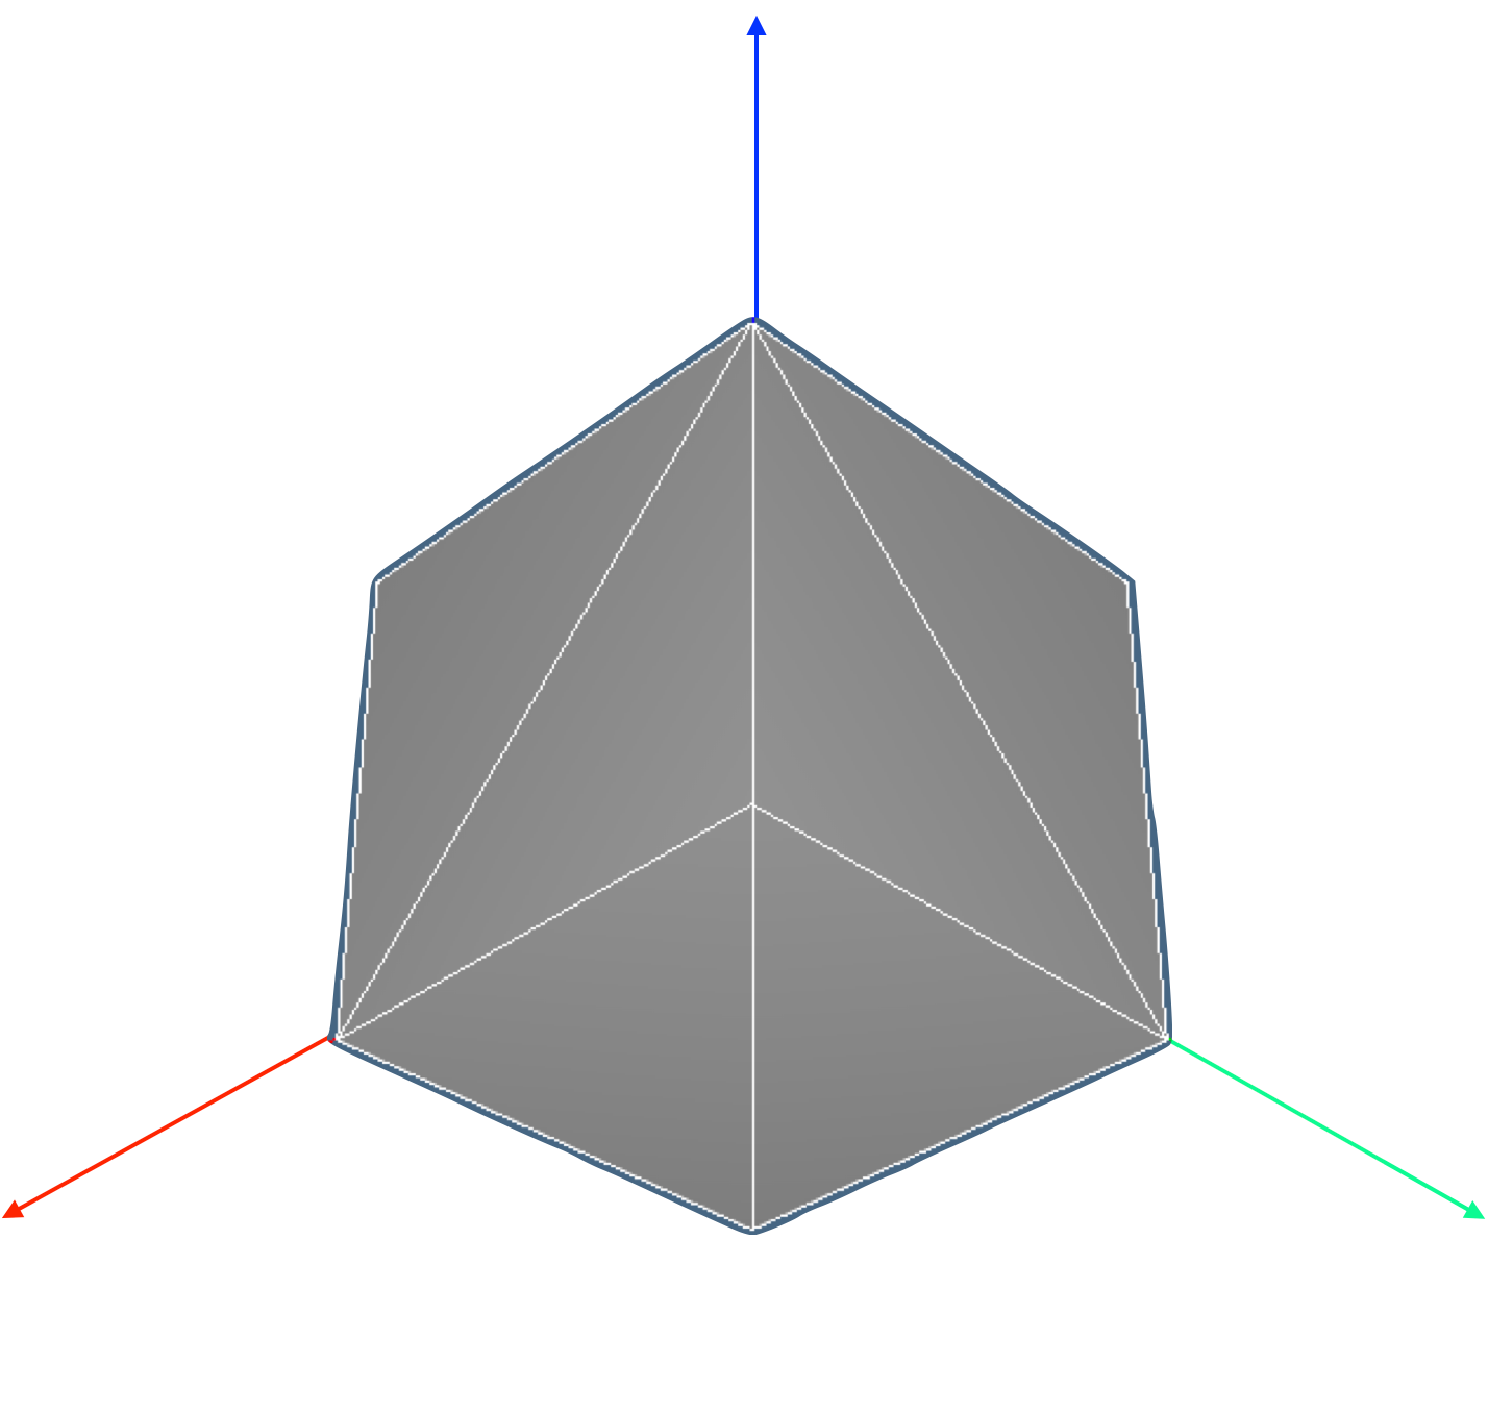
\includegraphics[width=2in]{chapter-04/figs/GRcube} 
\end{minipage}
\hfill
\begin{minipage}[c]{0.55\textwidth}
\begin{lstlisting}[language=JuliaLocal, style=julia, mathescape=true]
rotated = GR([1,1,1],π/3)(CUBE(1))
VIEW(rotated)
\end{lstlisting}
\caption{General rotation (GR) of angle $\pi/3$ about axis [1,1,1]. }
\end{minipage}
\end{figure}


\begin{coding}[General 3D rotation tensor]
In what follows, |MAT| transforms a Julia |Matrix| into a |Plasm| tensor applicable to |Hpc| values. 
The |HOMO| function apply to  a square matrix, adding new unitary first row and column, for homogeneous coordinates (see Section~\ref{}).  
\begin{lstlisting}[language=JuliaLocal, style=julia, mathescape=true]
GR(d,α) = MAT(HOMO(Q(d)')) ∘ R(1,2)(α) ∘ MAT(HOMO(Q(d)))
\end{lstlisting}
The |GR| (general rotation) is a |Plasm| tensor depending on the axis |d| and the angle |$\alpha$|. 
Our geometric model is therefore rotated and viewed as follows.
\end{coding}



\subsection*{Scaling}\label{sect:4-2-2}

In a scaling transformation, all points are moved along the line passing for the origin they belong to.  The scaling is said \emph{elementary} when only one of the coordinates changes. There are two scaling parameters $s_x, s_y$ in 2D geometry and three scaling parameters $s_x, s_y, s_z$ in 3D, to be used in scalar products by the point coordinates.
The transformation can be a \emph{dilatation} of space when scaling parameters are greter than one, or a \emph{contraction} of space when scaling parameters are lesser than one.
\[
S(s_x,s_y,s_z) = \mat{s_x & 0 & 0\\ 0 & s_y & 0\\ 0 & 0 & s_z},\ 
S_x = \mat{s_x & 0 & 0\\ 0 & 1 & 0\\ 0 & 0 & 1},\ 
S_y = \mat{1 & 0 & 0\\ 0 & s_y & 0\\ 0 & 0 & 1},\ 
S_z = \mat{1 & 0 & 0\\ 0 & 1 & 0\\ 0 & 0 & s_z} 
\]
The scaling matrices are diagonal.
The origin remains fixed. In fact: \[S\,\vet{0 &0 & 0}^t = \vet{0 & 0 & 0}^t.\] 
Hence, a scaling transformation is linear. It is easy to see that  scale transformations are multiplicative, commutative, and associative because the matrix is diagonal:
\[
\T{S}(s_x, s_y, s_z) = \T{S}_x(s_x)\, \T{S}_y(s_y)\, \T{S}_z(s_z)$.
\]
\begin{coding}[How to scale a Plasm model?]
As in the previous coding example, let’s go to use the |cube(1)| as our model object.

\begin{lstlisting}[language=JuliaLocal, style=julia, mathescape=true]
scaledcube1 = S(1,2,3)(.1,.1,10)(CUBE(1))
scaledcube2 = S(3)(100)(CUBE(1))
\end{lstlisting}
\end{coding}


\begin{coding}[How to scale a Plasm model?]
Note that the effect of transformations impacts only the homogeneous matrices ahead of |Hpc| values. 
\begin{lstlisting}[language=JuliaLocal, style=julia, mathescape=true]
scaledcube1 = S(1,2,3)(.1,.1,10)(CUBE(1)) 	#=
Hpc(MatrixNd([[1.0, 0.0, 0.0, 0.0], [0.0, 0.1, 0.0, 0.0], [0.0, 0.0, 0.1, 0.0], [0.0, 0.0, 0.0, 10.0]]), Hpc(MatrixNd(4), Hpc(MatrixNd(4), Geometry([[0.0, 0.0, 0.0], [1.0, 0.0, 0.0], [0.0, 1.0, 0.0], [1.0, 1.0, 0.0], [0.0, 0.0, 1.0], [1.0, 0.0, 1.0], [0.0, 1.0, 1.0], [1.0, 1.0, 1.0]], hulls=[[1, 2, 3, 4, 5, 6, 7, 8]])))) =#
scaledcube2 = S(2)(100)(SQUARE(1)) 	#=
Hpc(MatrixNd([[1.0, 0.0, 0.0], [0.0, 1.0, 0.0], [0.0, 0.0, 100.0]]), Hpc(MatrixNd(3), Hpc(MatrixNd(3), Geometry([[0.0, 0.0], [1.0, 0.0], [1.0, 1.0], [0.0, 1.0]], hulls=[[1, 2, 3, 4]])))) =#
\end{lstlisting}
Of course, |S(1,2,3)(.1,.1,10)| and |S(2)(100)| are tensor objects.
\end{coding}


\begin{coding}[Construction of octahedron model]
As an exciting coding example, we show a simple construction of an octahedron model, starting from the 3D SIMPLEX model.
\begin{lstlisting}[language=JuliaLocal, style=julia, mathescape=true]
tetra = SIMPLEX(3);
twotetra = STRUCT( tetra, S(1)(-1), tetra );
fourtetra = STRUCT( twotetra, S(2)(-1), twotetra );
octahedron = STRUCT( fourtetra, S(3)(-1), fourtetra );
\end{lstlisting}

Looking at the whole cellular complex corresponding to the solid model |octahedron::Hpc| is worthwhile. For this purpose, we transform it into an object of |Lar| type:

\begin{figure}[htbp] %  figure placement: here, top, bottom, or page
\begin{minipage}[c]{0.35\textwidth}
   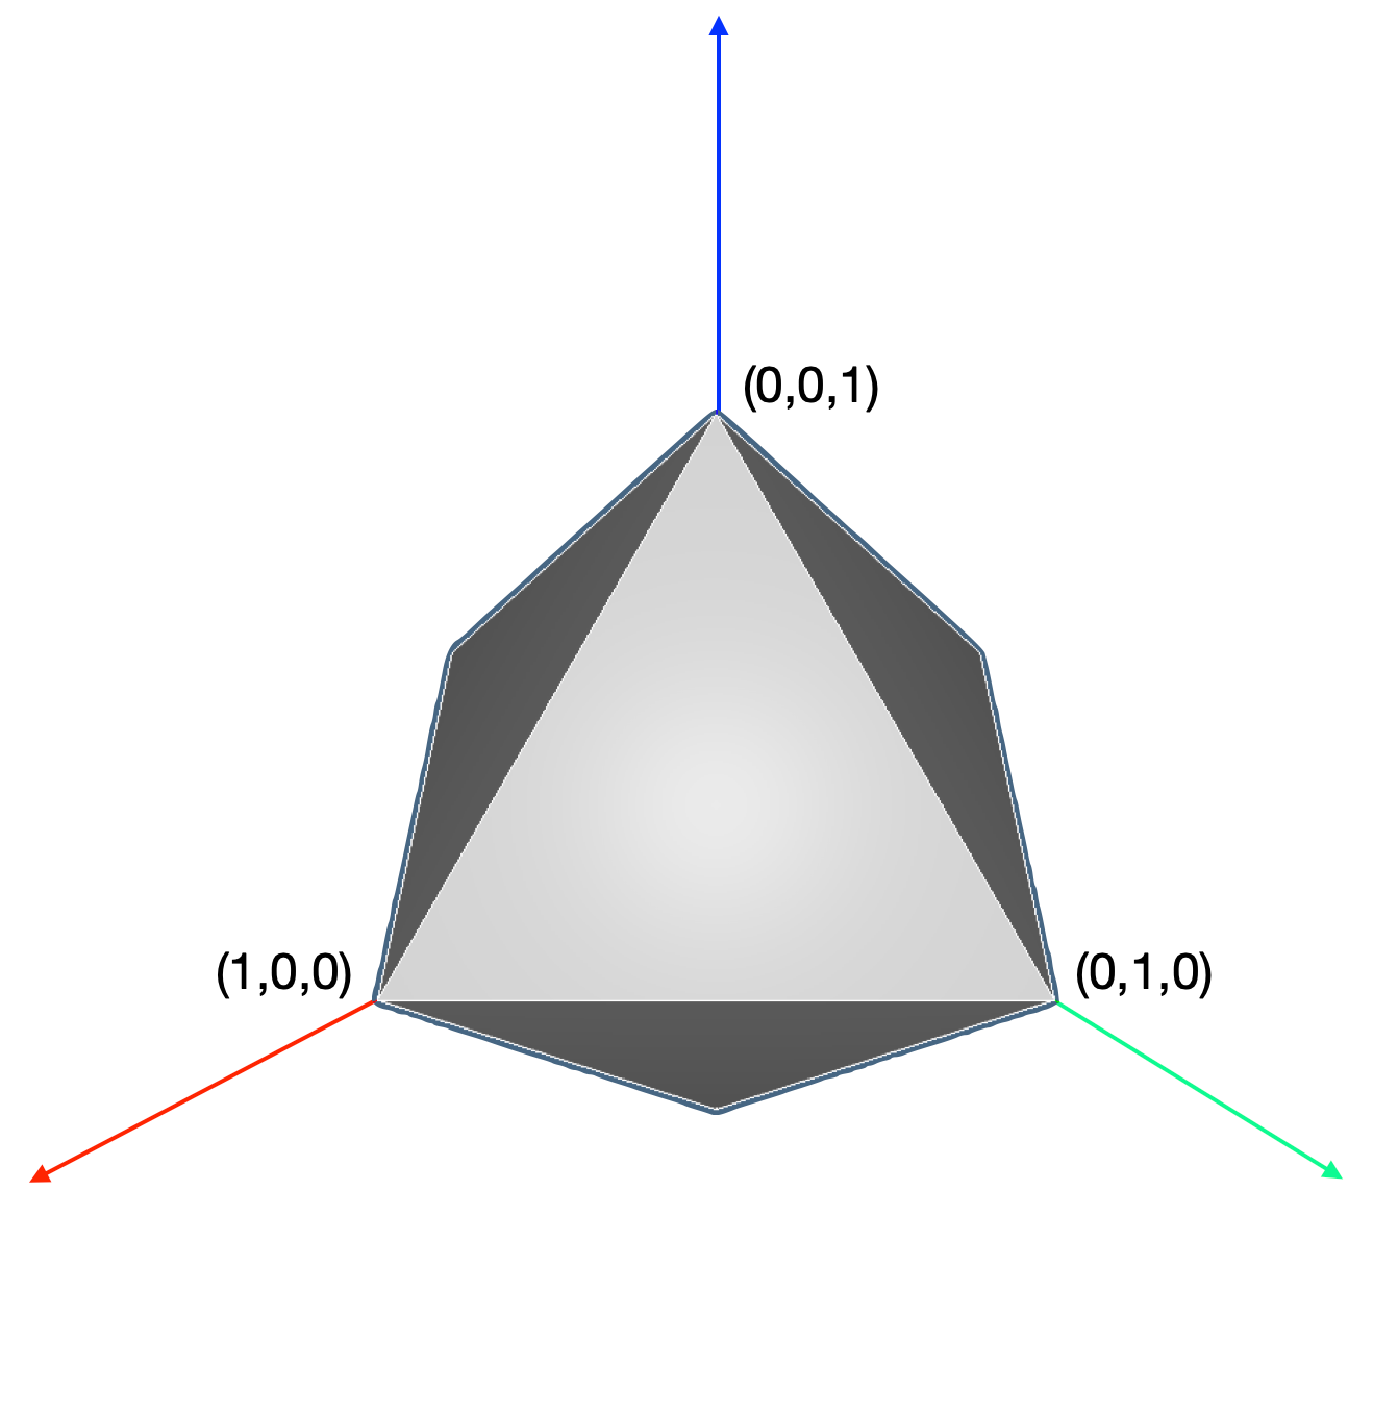
\includegraphics[width=\linewidth]{chapter-04/figs/octahedron} 
\end{minipage} \hfill
\begin{minipage}[c]{0.6\textwidth}
\begin{lstlisting}[language=JuliaLocal, style=julia, mathescape=true]
VIEW(octahedron::Hpc)
\end{lstlisting}
\caption{Plasm viewing generator expression. Remember that VIEW applies to Hpc values.}\label{fig:octahedron}
\end{minipage}
\end{figure}

\begin{coding}[The cellular complex]
Let’s note that the |octahedron::Hpc| is viewed, and that the |octahedron::Lar| is explored for stored data:\\
\begin{lstlisting}[language=JuliaLocal, style=julia, mathescape=true]
LAR(Octahedron).V 	#=
3×7 Matrix{Float64}:
  0.0  -1.0  0.0   0.0  1.0  0.0  0.0
 -1.0   0.0  0.0   0.0  0.0  1.0  0.0
  0.0   0.0  0.0  -1.0  0.0  0.0  1.0 	=#
LAR(Octahedron).C	#=
Dict{Symbol, AbstractArray} with 3 entries:
  :CV =) [[1, 2, 3, 4], [1, 3, 4, 5], [2, 3, 4, 6], [3, 4, 5,…
  :FV =) [[1, 2, 3], [2, 3, 4], [1, 3, 4], [1, 2, 4], [1, 3, …
  :EV =) [[2, 3], [1, 3], [1, 2], [3, 4], [2, 4], [1, 4], [3,…=#
\end{lstlisting}

For |$\#$C, $\#$F, $\#$E, $\#$V|, we see, looking at |.V| and |.C| above:
\begin{lstlisting}[language=JuliaLocal, style=julia, mathescape=true]
AA(LEN)(values(octahedron.C))'	#=
1×3 adjoint(::Vector{Int64}) with eltype Int64:
 8  20  18		=#
\end{lstlisting}
Therefore, we may see that the combinatorial (simplicial) complex corresponding to the 3D octahedron is made by 
8 + 20 + 18 + 7 = 53 cells of dimension 3, 2, 1, and 0, respectively (see Figure~\ref{fig:octahedron}).
\end{coding}




\subsection*{Shearing}
\label{s*ec:ccccccc}

In  a 2D elementary \emph{shearing tranformation} all points of each line (plane in 3D) orthogonal to a coordinate axis move by summing one (fixed) vector. The coordinate line (plane in 3D) remain fixed, and the translation vector change linearly with the distance of its line (plane) from the origin. Each of two elementary planar shearing depends on a single scalar parameter (the translation of the line at unit distance from the coordinate line). 

Each of the three elementary space shearing in 3D conversely depends on two scalar parameters (the coordinates of the planar translation vector of the plane at unit distance from the coordinate plane. Their 2D  and 3D matrices are as follows.

\[
\T{H}_x(h_x) = \mat{1\  & 0\\h_x & 1 },\qquad
\T{H}_y(h_y) = \mat{1\  & h_y\\0 & 1 };
\]
\[
\T{H}_x(h_y,h_z) = \mat{1 & 0 &  0 \\h_y & 1 & 0\\h_z & 0 & 1},\ 
\T{H}_y(h_x,h_z) = \mat{1 & h_x & 0 \\0 & 1 & 0\\0 & h_z & 1},\ 
\T{H}_z(h_x,h_y) = \mat{1 &  0 &  h_x\\0 & 1 & h_y\\0 & 0 & 1}.
\]

An elementary shearing differs from the identity matrix only for the elements of a single column, both in 2D and in 3D, and also in homogeneous 4D coordinates. 
In |Plasm|, the shearing tensor is named |H| and has the following semantics: first, indicate the column index; then give the $d-1$ ordered transformation parameters, i.e., one in 2D and two in 3D, some of which possibly zeros. Therefore we have |H(col)(pars)|.

\begin{figure}[htbp] %  figure placement: here, top, bottom, or page
\begin{minipage}[c]{0.35\textwidth}
   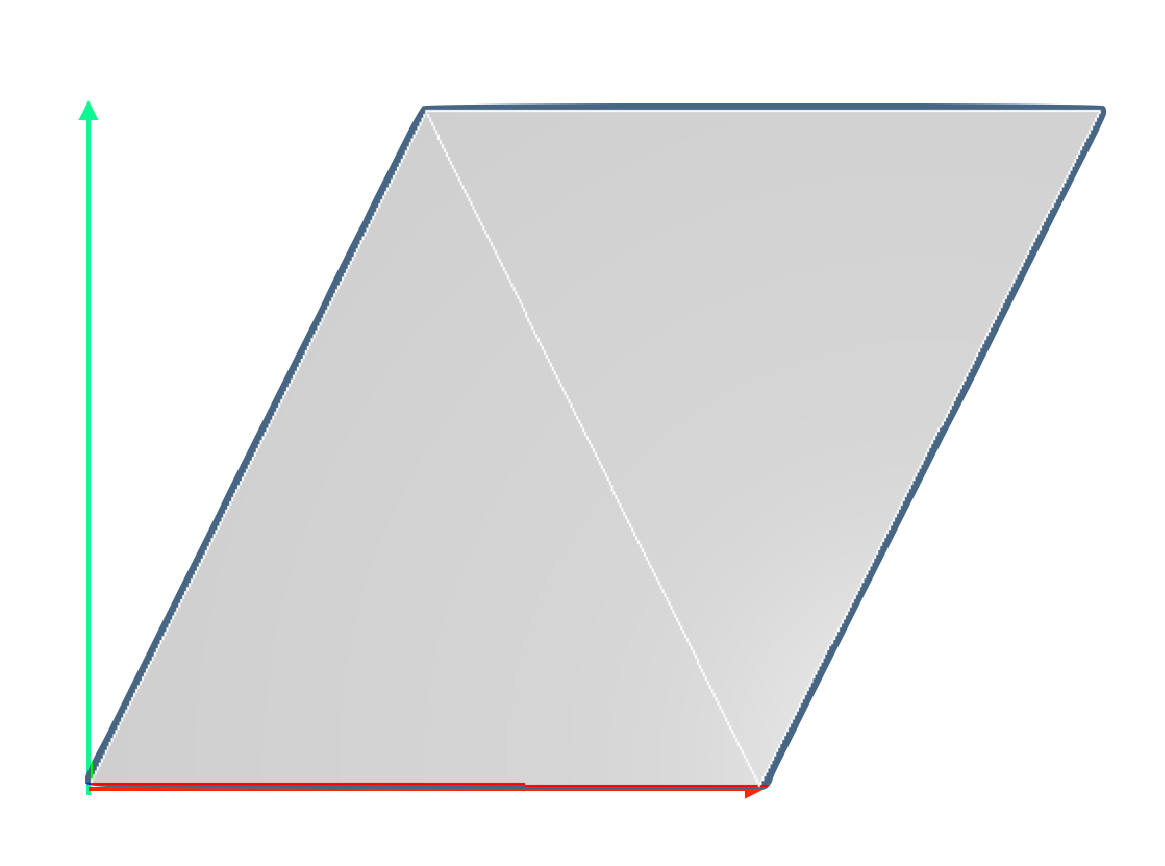
\includegraphics[width=\linewidth]{chapter-04/figs/shear2D} 
\end{minipage}\hfill
\begin{minipage}[c]{0.60\textwidth}
\begin{lstlisting}[language=JuliaLocal, style=julia, mathescape=true]
SQUARE(d) = CUBOID([d,d])
shearedsquare = H(2)(.5)(SQUARE(1))

VIEW(shearedsquare)
\end{lstlisting}
   \caption{Unit square sheared on the (second) coordinate $y$. The $y$ of model points does not change.}
\end{minipage}
\end{figure}

Typically, |shearing| is used by typesetting systems of computerized typography to get \emph{italic} versions of character fonts. Note also above how we define a parametric square (with a vertex on the origin).

\begin{figure}[htbp] %  figure placement: here, top, bottom, or page
\begin{minipage}[c]{0.35\textwidth}
   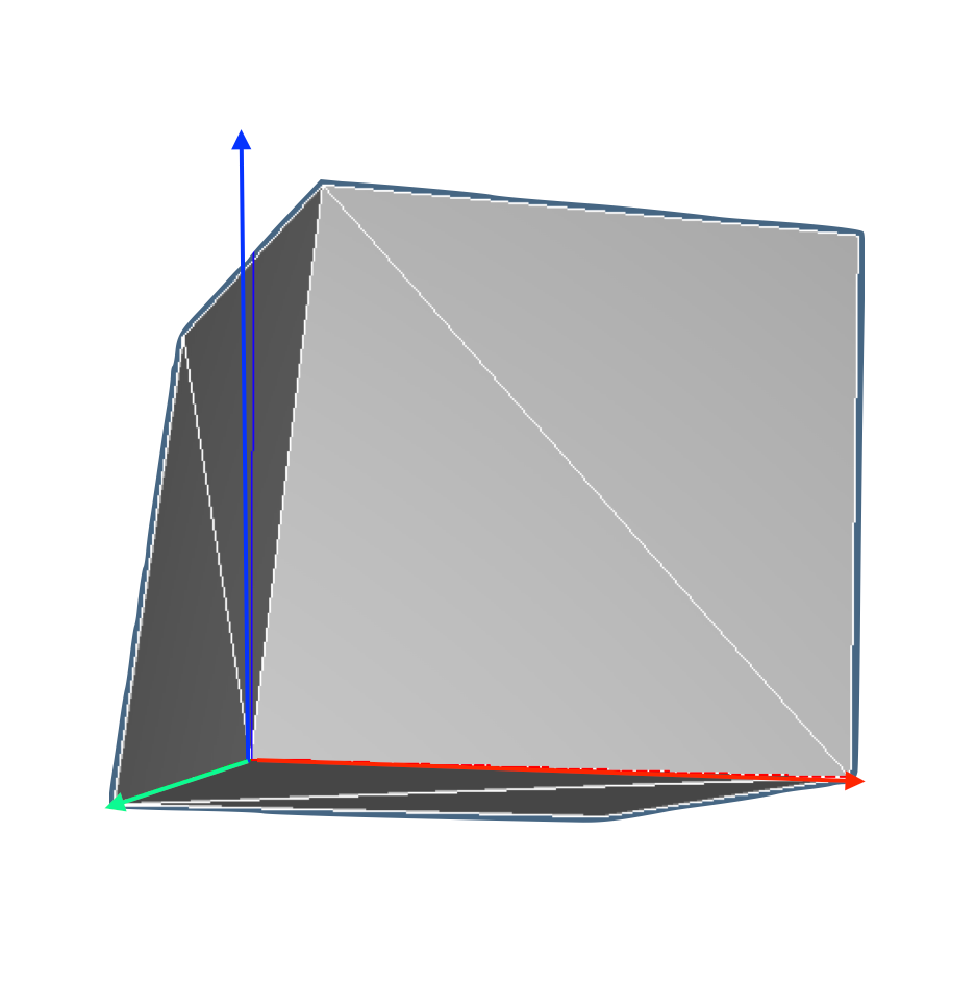
\includegraphics[width=\linewidth]{chapter-04/figs/shear3D} 
\end{minipage}\hfill
\begin{minipage}[c]{0.60\textwidth}
\begin{lstlisting}[language=JuliaLocal, style=julia, mathescape=true]
shearedcube = H(3)(.2,.3)(CUBE(1))

VIEW(shearedcube)
\end{lstlisting}
   \caption{Unit cube sheared on the (third) coordinate $z$. The $z$ of points do not change.}
\end{minipage}
\end{figure}

It is worthwhile to remark that the |H| mapping, as |R|, |GR|, |S|, |T|, |MAT|, and |HOMO| are dimension-independent, so can be applied to models of whatever embedding dimension $d$ of geometric models. Homogeneous \emph{normalized} matrices are used for implementation purpose. 


 
\subsection*{Translation}
\label{subsec:2:translation}

\begin{definition}[Translation transformation]
a translation is an invertible transformation of Euclidean space $\E^d$ generated by summing a fixed vector to all points.

A translation of plane $\mathbb{E}^2$ (or space $\mathbb{E}^3$) is not a linear transformation, since it moves the origin, but it is an \emph{affine} transformation, since all $\mathbb{E}^2$ (or $\mathbb{E}^3$) mapped points change by sum with a fixed vector (an \emph{affine action}). 
\end{definition}

Hence, a 2D or 3D translation depends on two (or three) scalar parameters, i.e., by the coordinates of the \emph{translation vector}.
We may therefore translate, using coordinates, a generic vector $\v{v} = (v_i)\in\mathbb{E}^d$:
\begin{equation}
\v{v}’ = \v{v} + \v{t}
\label{eq:vectortranslation}
\end{equation}
where $\v{t} = ({t}_i)$ is the translation vector, applied to all points in $\mathbb{E}^d$.




\subsubsection*{Translation in homogeneous coordinates}

The translation \ref{eq:vectortranslation} is reduced to a linear transformation and hence is representable by a product with a square matrix when using normalized homogeneous coordinates. Let’s remind our choice to use as homogeneous the first coordinate. 
For example, a translation of $\mathbb{E}^3$ is representable as
\begin{equation}
\T{T}(t_x,t_y,t_z) = \mat{1 & 0 & 0 & 0\\t_x & 1 & 0 & 0\\t_y & 0 & 1 & 0\\t_z & 0 & 0 & 1}
\end{equation}

We can see the equivalence between translation with Cartesian coordinates and homogenous normalized (affine) coordinates. Let $\v{v} = (x,y,z)$ be a point in 3D Euclidean space $\mathbb{E}^3$, and $\v{v}’ = (w=1,x,y,z)$ the same point in $\mathbb{R}^4$:
\[
\vet{x\\y\\z} + \vet{t_x\\t_y\\t_z} = \vet{x+t_x\\y+t_y\\z+t_z}
\qquad\mbox{and}\qquad
\mat{1 & 0 & 0 & 0\\
	t_x & 1 & 0 & 0\\
	t_y & 0 & 1 & 0\\
	t_z & 0 & 0 & 1} \, 
	\vet{1\\x\\y\\z} = \vet{1\\x+t_x\\y+t_y\\z+t_z}
\]

Just notice that a translation in 3D is actually a shearing $H_w(t_x,t_y,t_z)$ orthogonal to the added component in normalized homogeneous coordinates.

\begin{coding}[Translation of 3D geometric object] 
In |Plasm| we translate a geometric object of |Hpc| type via tensor application:

\begin{lstlisting}[language=JuliaLocal, style=julia, mathescape=true]
t_cube1 = T(1,2,3)(.5,.5,.5)(CUBE(1))
t_cube2 = T(3)(1)(CUBE(1))

VIEW(t_cube1);  VIEW(t_cube2)
\end{lstlisting}
A triple application of |T| function is needed: first to indices, then to translation paramenters, finally to the object of |Hpc| type to be translated.
\end{coding}

\begin{coding}[Parametric linear ladder stair] 
The |step| is a |Hpc| solid obtained by product of three line segments of given sizes.
An array of $n$ pairs |[move, step]| is generated and concatenated by the |CAT| operator.  Finally, the semantics of |STRUCT| aggregator combinator (see Section~\ref{sect:4-3}) produces the whole parametric object, shown in Figure~\ref{fig:stair}. 

\begin{lstlisting}[language=JuliaLocal, style=julia, mathescape=true]
function Ladder(lx,ly,lz, n)::Hpc
	step   = QUOTE(lx) * QUOTE(ly) * QUOTE(lz)
	move   = T(2,3)(0.8*ly, 0.8*lz)
	ramp   = STRUCT( CAT([[step, move] for k=1:n]) )
end #=
Ladder (generic function with 1 method)	=#
stair = Ladder(.8, .22, .18, 15);

VIEW(stair)
\end{lstlisting}

\end{coding}



\begin{figure}[htbp] %  figure placement: here, top, bottom, or page
   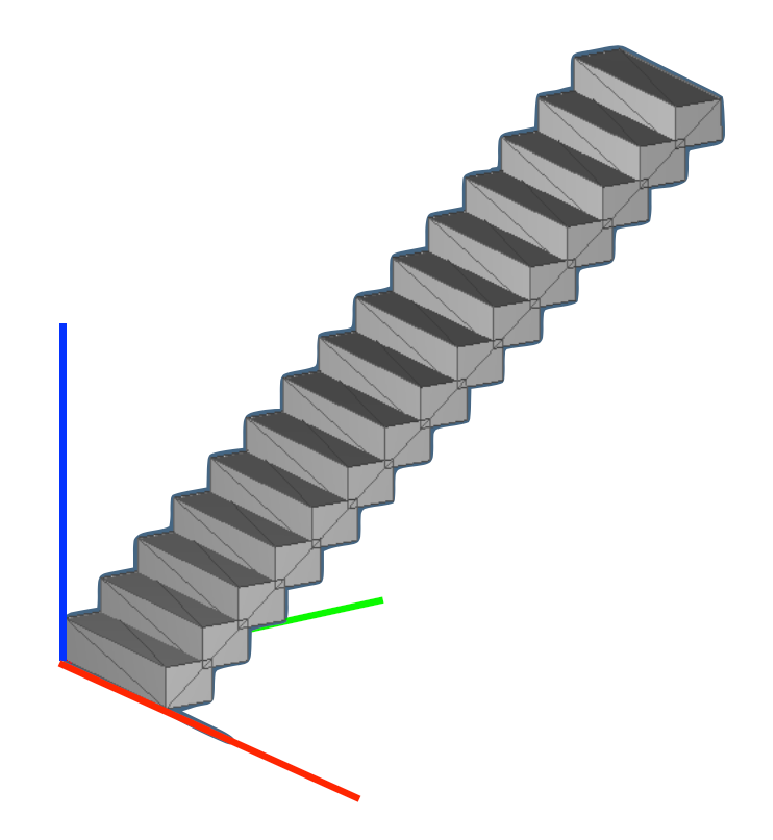
\includegraphics[width=0.35\linewidth]{chapter-04/figs/stair}
   \hspace{5mm}
   \sidecaption[t]
   \caption{Simple linear scale, demostrating an iterative use of tensors in {\small\sf STRUCT}. Of course, not only the number, but also the size and even the shape of {\sf step} model can be parametrized, as arguments of a geometric function returning {\sf Hpc} objects.}
   \label{fig:stair}
\end{figure}  






\section{Assembly of geometric objects}\label{sect:4-3}

Complex shapes are usually defined as hierarchical assemblies of either geometric primitives or more  complex shapes, each defined in a local coordinate system. 

Most graphics and modeling systems implement this semantics as a tree or \emph{hierarchical graph}, where affine geometry within the \emph{nodes} is defined in local coordinate frames, and arcs are associated to affine transformations that move the whole subgraph rooted in the ending node onto the coordinate system of the first node of the arc. The very first node is called \emph{root} of the data structure.


\subsection{Hierarchical graphs}

Acyclic graphs/multigraphs are also called \emph{hierarchical graphs}, because can be associated to a tree, generated at run-time by visiting the graph with some standard traversal algorithm~\cite{10.5555/1614191}, e.g., with a depth-first-search (DFS).  The ordered sequence of nodes produced by the traversal is sometimes called a \emph{linearized graph}.  Each node in this sequence is suitably transformed from local coordinates to \emph{world coordinates}, i.e. to the coordinates of the root, by the traversal algorithm.

The main ideas concerning \emph{scene graphs} can be summarized as
follows.
Nodes are  \emph{containers} of geometrical datasets stored in
\emph{local} coordinates.  Nodes are also used and implemented as root of subgraphs, 
whose data are transformed to the node coordinates by a traversal
algorithm.
Arcs $(a,b)$ are associated with affine transformations, which map the
data contained in $b$ from their local coordinates to the coordinates
of $a$.  More than one arc may exist between the same node pair.  This
allows storage in memory only of \emph{one copy} of each container.
The composite transformations of coordinates applied to the linearized
graph generated at traversal time are collectively known as the
\emph{modeling transformation}.


\subsection*{Object Transform}\label{sect:4-3-1} Any |Plasm| geometric value of |Hpc| type can be affinely transformed by direct application of an affine tensor to it.

\begin{coding}[Direct use of Tensor]\ 
Let’s combine with other language tensors, while generating the translated 1-skeleton of a cube:
\begin{lstlisting}[language=JuliaLocal, style=julia, mathescape=true]
SK = SKELETON;
translatedcube = (SK(1) ∘ T(1)(1) ∘ CUBE)(1);
\end{lstlisting}
\end{coding}

\begin{coding}[Example.2]\ 
Then, aggregate two objects into a single object within the \emph{same} coordinate frame:
\begin{lstlisting}[language=JuliaLocal, style=julia, mathescape=true]
singleframe = STRUCT(cube, tetra);
VIEW(singleframe)
\end{lstlisting}
\end{coding}

\begin{coding}[Example.3]\ 
\emph{Direct} application of tensor |T$_z$(1)|, followed by application of |R$_z$(-π/2)| to |tetra| value, which changes accordingly:
\begin{lstlisting}[language=JuliaLocal, style=julia, mathescape=true]
doubleframes = STRUCT(cube, (R(1,2)(-π/2) ∘ T(3)(1.0))(tetra) 
VIEW(doubleframes)
\end{lstlisting}
\end{coding}

\begin{coding}[Example.4]\ 
Exactly the same effect could be obtained by the following expression, because \emph{a transformation tensor is implicitly applied to every geometric value following it} in the parameter sequence of a |STRUCT| combinator. Evaluation is right-to-left, according to math composition rule:
\begin{lstlisting}[language=JuliaLocal, style=julia, mathescape=true]
doubleframe = STRUCT(cube, R(1,2)(-π/2), T(3)(1), tetra )
\end{lstlisting}
\end{coding}

\subsection*{Assembly of components}\label{sect:4-3-2}

Hierarchical models of complex assemblies are generated by aggregation of cellular complexes, each one defined in a local coordinate system, and possibly
relocated by affine transformations of coordinates.  This operation may be repeated
hierarchically, with subassemblies defined by aggregation of simpler parts, and so
on, until to have a set of leaves holding primitive models, which cannot be further decomposed.

Two main advantages can be found in a hierarchical modeling approach. Each component complex  and each partial assembly, at every hierarchical level, are defined independently from each other, using their |PROPERTIES| and local coordinate frame, suitably chosen to make the  definition easier.
Furthermore, only one copy of each component is stored in memory, and may be instanced
in different locations and orientations how many times it is needed.

\begin{figure}[htbp] %  figure placement: here, top, bottom, or page
   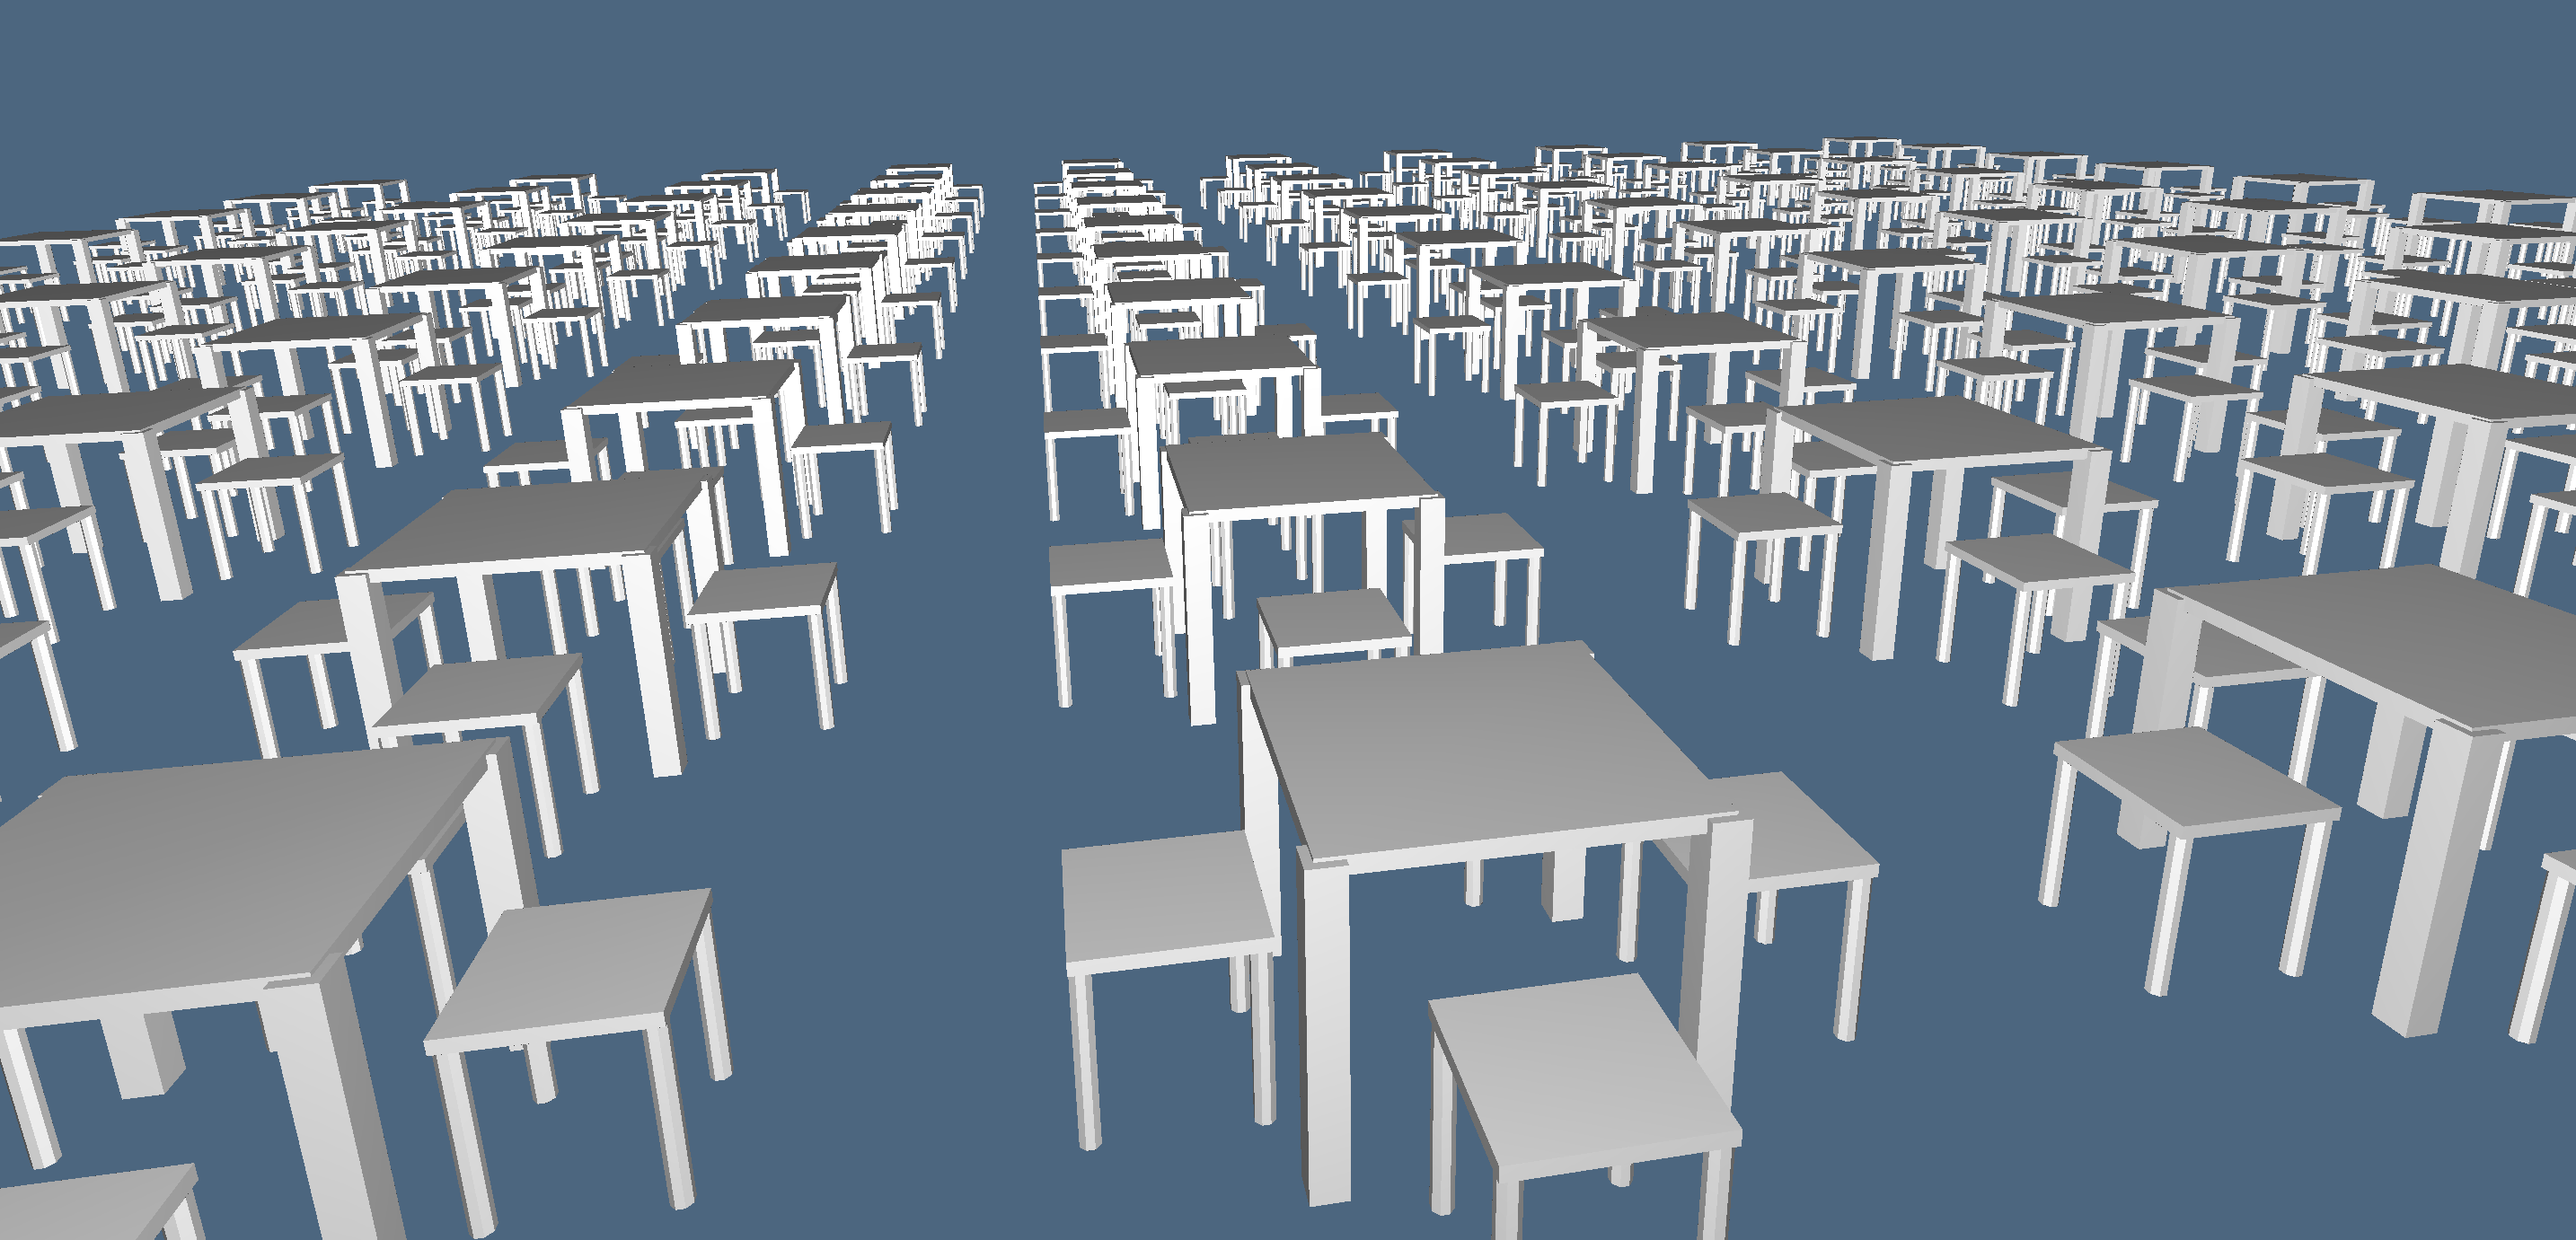
\includegraphics[width=\linewidth]{chapter-04/figs/refectory.png}
   \hspace{5mm}
   \caption{Hierarchical assembly of cellular 3-complexes.}
   \label{fig:refectory}
\end{figure}  


\subsubsection*{Directed Acyclic Graph (DAG)}\label{sect:4-3-2-1}

A \emph{hierarchical model}, defined inductively as an assembly of component parts,
is described by an \emph{acyclic directed multigraph}, often called a \emph{scene graph} or \emph{hierarchical structure} in computer graphics and modeling.  The main algorithm with hierarchical assemblies is the \emph{traversal} function, which transforms every component of the assembly from \emph{local coordinates} to global coordinates, often called \emph{world coordinates}.

\begin{definition}[Directed graph] A directed graph $G$ is a pair $(N,A)$, where
$N$ is a set of \emph{nodes} and $A$ is a set of directed \emph{arcs}, given as ordered pairs of nodes.  
\end{definition}
Such a definition is not sufficient when more than one arc must be considered
between the same pair of nodes.
The notion of \emph{multigraph} is hence introduced.  
In a multigraph, the same pair of nodes can be connected by multiple arcs.

\begin{definition}[Directed multigraph] A directed multigraph is a
triplet $G := (N,A,f)$ where $N$ and $A$ are sets of nodes and arcs, respectively, and $f:
A \to \mathbf{N}^{2}$ is a mapping from arcs to node pairs.  
\end{definition}

Directed graphs or multigraphs are said to be \emph{acyclic} when they do not contain cycles, i.e. when no path starts and ends at the same vertex.  \emph{Trees} are common examples of acyclic graphs. A tree, where each non-leaf node is the root of a subtree, is the best model of the concept of \emph{hierarchy}. Nodes in a tree can be associated with their integer \emph{distance} from the root, defined by the number of edges on the unique path from the root to the node.  A tree can be layered by \emph{levels}, by putting in the same subset (level) all the nodes with equal distance from the root.

\subsubsection*{Hierarchical structures in Plasm}\index{Hierarchical!structures in Plasm}


A \emph{container} of geometrical objects is defined in |Plasm| by
applying the combinator |STRUCT| to the contained objects' sequence (or array).  The value returned from the function application is of type 
\emph{hierarchical polyhedral complex} |Hpc|.  The coordinate system used by
the returned value is the one associated with
the first geometric object of the argument sequence.  

The resulting geometrical value is often associated with a variable used as the container's name, as in
\begin{lstlisting}[language=JuliaLocal, style=julia, mathescape=true]
    obj = STRUCT( obj$_{1}$, obj$_{2}$, $\ldots$, obj$_{n}$ ); VIEW(obj)
\end{lstlisting}

The |obj| geometry can be pictorially described, using the
previously discussed graph model of hierarchical structures, as shown
in Figure~\ref{fig:4:struct1}a.  Clearly, each component object may in
turn be defined as a container of other objects, i.e.~as the root of a
subgraph, as shown as shown below:
\begin{lstlisting}[language=JuliaLocal, style=julia, mathescape=true]
    obj$_2$ = STRUCT( obj$_{21}$, $\ldots$, obj$_{2m}$ )
\end{lstlisting}


\begin{figure}[htbp] %  figure placement: here, top, bottom, or page
   \centering
   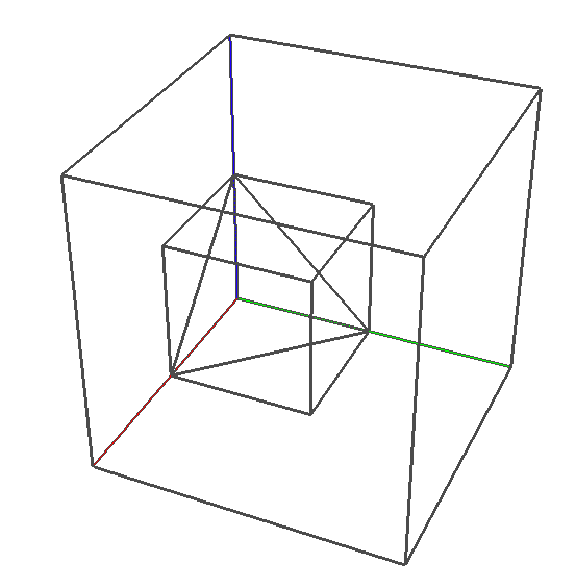
\includegraphics[width=0.3\linewidth]{chapter-04/figs/global} 
   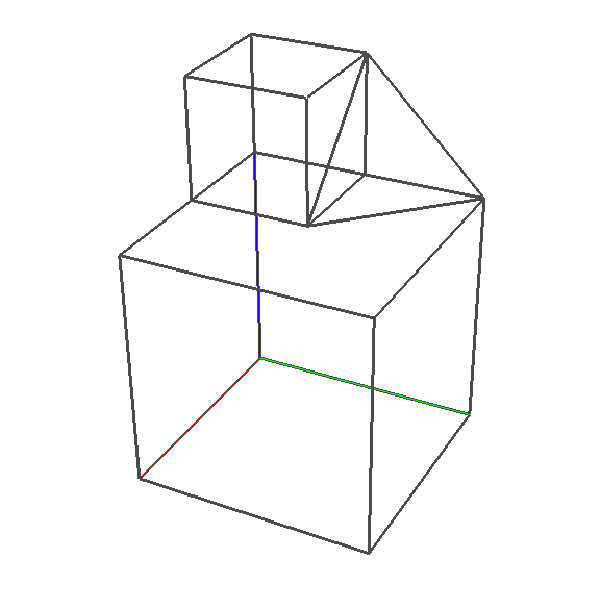
\includegraphics[width=0.3\linewidth]{chapter-04/figs/local} 
   \caption{Assembly by STRUCT: (a) without coordinate transformations. All three objects have the same origin;
    (b) with coordinate transformations.}
   \label{fig:4:struct1}
\end{figure}

Exactly the same geometric result would be generated by direct nesting of |STRUCT|
sub-expressions:
\begin{lstlisting}[language=JuliaLocal, style=julia, mathescape=true]
obj = STRUCT(obj$_1$, STRUCT(obj$_{21}$, $\ldots$, obj$_{2m}$) $\ldots$, obj$_n$)
\end{lstlisting}


The sequence argument of the |STRUCT| operator may either
contain or not affine transformations, together with polyhedral
complexes.  This fact results in generating an assembly either by
using the same (global) coordinates for the various components or by
using different (local) coordinate systems.  The two cases are
discussed in the two following subsections, respectively.

\subsubsection*{Assembly with global vs local coordinates}

Let’s assume that the sequence argument of a |STRUCT| expression
does not contain affine transformations. In other words, we assume
that the evaluations of the Plasm expressions in the argument sequence
only return polyhedral values.
In this case, the output polyhedral complex is returned within the
coordinate frame of the first element of the input sequence, and no
transformations of coordinates are applied to the assembly components,
which are only aggregated in the same space, as shown by the
the following example.

\begin{coding}[STRUCT assembly (1)]
The expression given below returns the
object of Figure~\ref{fig:4:struct1}a.  Note that the
three component shapes' local origin and coordinate axes
coincide.  The |SK(1)| operator (extraction of 1-skeleton)
was |$@1$|, not available in Julia, in classic |PlaSM|).
    
\begin{lstlisting}[language=JuliaLocal, style=julia, mathescape=true]
cube2, cube1, simplex = CUBE(2), CUBE(1), SIMPLEX(3)
obj1 = (SK(1) ∘ STRUCT)( cube2, cube1, simplex )
\end{lstlisting}
%obj1 = PROPERTIES(obj, Dict("line_width"=)3))
%VIEW(obj, Dict("background_color"=)[1,1,1]))
\label{ex:8:globalcoords}    
\end{coding}


\begin{coding}[STRUCT assembly (2)] \label{coding:4:2}
Here we aggregate the same geometric components used in
Coding~\ref{ex:8:globalcoords}, but also add up some
transformations of coordinates to the sequence of parameters of resulting assembly.
\begin{lstlisting}[language=JuliaLocal, style=julia, mathescape=true]
obj2 = (SK(1) ∘ STRUCT)(cube2, T(3)(2), cube1, T(2)(1), simplex)
\end{lstlisting}
%obj = PROPERTIES(obj, Dict("line_width"=)3))
%VIEW(obj, Dict("background_color"=)[1,1,1]))
\label{ex:8:localcoords}
The resulting geometric assembly is shown in \ref{fig:4:struct1}b.  
\end{coding}


\subsection*{STRUCT semantics}
\label{sec:8:localcoords}

We assume that in |Plasm|, the word \emph{tensor} stands for affine transformation.
Let’s suppose that tensors $|T|_k$ are contained
within the sequence argument of a |STRUCT| expression.
Each tensor in a |STRUCT| is applied to all polyhedral
complexes that follow it. The subsequent expressions are equivalent:

\begin{lstlisting}[language=JuliaLocal, style=julia, mathescape=true]
STRUCT( pol$_{1}$, T$_{1}$, pol$_{2}$, T$_{2}$, pol$_{3}$, $\ldots$ , T$_{n-1}$, pol$_n$ ) $\equiv$ 
STRUCT( pol$_{1}$, T$_{1}$(pol$_{2}$), (T$_{1}$$\sim$T$_{2}$)(pol$_{3}$), $\ldots$, (T$_{1}$∘T$_{2}$$∘\cdots∘$T$_{n-1}$)(pol$_{n}$)
\end{lstlisting}

Looking at the internal behavior of the geometric kernel of the
language, the following maps are applied to the |STRUCT|
application at evaluation time:

\begin{lstlisting}[language=JuliaLocal, style=julia, mathescape=true]
STRUCT( pol$_{1}$, (T$_{1}$ ∘ STRUCT)( pol$_{2}$, (T$_{2}$ ∘ STRUCT)( pol$_{3}$, $\ldots$ 
	(T$_{n-2}$ ∘ STRUCT)( pol$_{n-1}$, T$_{n-1}$(pol$_{n}$) ) $\ldots$ ) ) )
\end{lstlisting}

The above kind of evaluation (in DFS postorder) has inspired the actual implementation of the |Hpc| data structure.
Note, looking at the geometric result shown in
Figure~\ref{fig:4:struct1}b, that, according to Coding~\ref{coding:4:2}:
\begin{enumerate}
    \item
the output assembly is
represented in the coordinate system of first cube; 
    \item
the second cube is translated in $z$ direction; 
    \item
the unit tetrahedron is translated both in $z$ and in $y$ directions.
\end{enumerate}


\subsection*{Traversal algorithms}\label{sect:4-3-3}

There are many ways to visit (or walking) a graph or multigraph, traversing at least once every node or arc.
The \emph{traversal} of a hierarchical structure consists of a 
modified
\emph{Depth First Search} (DFS) of its acyclic multigraph,\footnote{
Notice that the standard \emph{dfs} graph traversal (see 
e.g.~\cite{AhoHopcroftUllman:DSA}) visits all the nodes once, since it works by
recursively visiting those sons of each node that it has not already 
visited. }
where each arc --- and not each node --- is traversed only once.  
% The
% traversal algorithm visits only one time all the edges, and is therefore executed in time
% \emph{linear} with the edge number.  Conversely, 
In particular, each node is traversed a number of times equal to the
number of different paths that reach it from the root node.

The aim of a traversal algorithm is to ``linearize" a 
structure network, by transforming all its substructures (i.e.~all the
subgraphs) from their \emph{local coordinates} to the coordinates of
the root node, assumed as \emph{world coordinates}.
% , as discussed in
% the following chapter, where the various coordinate systems used in a 
% \textsf{PHIGS}-like 3D pipeline are discussed.

For this purpose, a matrix denoted as the \emph{current transformation
matrix} (CTM) is maintained.  Such a CTM is equal to the product of
matrices associated with the arcs of the current path from the root to
the current node.  For the sake of efficiency, the traversal algorithm is
implemented by using a stack of CTMs.  When a new arc is traversed,
the old CTM is pushed on the stack, and a new CTM is computed by
(right) multiplication of the old one times the matrix of the arc. 
When unfolding from the recursive visit of the subgraph appended to the
arc,\footnote{Using a pictorial image, we could say: when the arc is
traversed in the opposite direction.} the CTM is substituted by the one
popped from the stack.  The \textsc{Traversal} algorithm is specified
in pseudo-language below.


\begin{script}[Traversal of a multigraph]
\begin{tabbing}
aaa\=aaa\=aaa\=aaa\=aaa\=aaa\=aaa\=aaa\=\kill
{\bf algorithm} \textsc{Traversal} ($(N,A,f): multigraph$) \+\\
   $CTM$ := identity matrix;\\
    TraverseNode ($root$)
\end{tabbing}


\begin{tabbing}
aaa\=aaa\=aaa\=aaa\=aaa\=aaa\=aaa\=aaa\=\kill
{\bf proc} \textsc{TraverseNode} ($n: node$) \+\\
  \textbf{foreach} $a\in A
  $ outgoing from $n$
  \textbf{do} \+\\
    TraverseArc ($a$); \\
  ProcessNode ($n$)
\end{tabbing}


\begin{tabbing}
aaa\=aaa\=aaa\=aaa\=aaa\=aaa\=aaa\=aaa\=\kill
{\bf proc} \textsc{TraverseArc} ($a=(n,m): arc$) \+\\ 
  Stack.push ($CTM$);\\
  $CTM$ := $CTM * a$.mat;\\
  TraverseNode ($m$);\\
  $CTM$ := Stack.pop()
\end{tabbing}



\begin{tabbing}
aaa\=aaa\=aaa\=aaa\=aaa\=aaa\=aaa\=aaa\=\kill
{\bf proc} \textsc{ProcessNode} ($n: node$) \+\\ 
  \textbf{foreach} object $\in$ $n$ \textbf{do} \+\\
    Process( $CTM * $object )
\end{tabbing}
\end{script}

\vspace{5mm}
The CTM is normally used to (left) multiply the vertices of geometric
objects stored in the traversed containers.  But the reader should
remember that equations of hyperplanes and normal vectors must be
conversely (right) multiplied for the inverse of the applied
transformation, according to the mapping of covectors discussed in
Section~\ref{subsec:6:actiononcovectors}.  A double stack of matrices,
where to push/pop both the CTM and its current inverse, may therefore
speed up the traversal.  As a result of the algorithm, a linearized model
in world coordinates is produced, which may be used, e.g., for rendering
purposes, as discussed in the next chapter.



\subsection*{Assembly examples}\label{sect:4-3-4}

The two examples given in this section are finalized to introduce some powerful |Plasm| higher-level functions and combinators. In particular, we use |STRUCT| and |MAP|, |CAT|, |DIESIS|, |PROPERTIES|, and |THINSOLID|. The geometric primitives |CUBE|, |CYLINDER|, and |SIMPLEX| are also used.

\subsubsection*{Refectory room model}\label{sect:4-3-4-1}

Some coordinated coding examples are given here, to show the development bottom-up of the geometric model of a refectory room with its main appliances, tables and user chairs. The room is visualized in Figure~\ref{fig:refectory}.

\begin{coding}[Table]\ 
Both the |tableTop| and |tablelegs| with $4$ |tableLeg| instances are generated starting from 3D cube of side 1:
\begin{lstlisting}[language=JuliaLocal, style=julia, mathescape=true]
cube = T(1,2)(-.5,-.5)(CUBE(1));
tableTop  = STRUCT( T(3)(.85), S(1,2,3)(1,1,.05), cube );
tableLeg  = STRUCT( T(1,2)(-.475,-.475), S(1,2,3)(.1,.1,.89), cube );
tablelegs = STRUCT( CAT(DIESIS(4)([tableLeg, R(1,2)(π/2)])) );
table = STRUCT( tableTop, tablelegs );
VIEW( table )
\end{lstlisting}
The operator |DIESIS| ($\#$) in old |Plasm| repeats 4 times its second argument.
\end{coding}

\begin{coding}[Chair]\ 
The |chair| object is made by a |chairTop| and 4 cylindrical |chairLeg| with radius |0.06| and height |0.5|:
\begin{lstlisting}[language=JuliaLocal, style=julia, mathescape=true]
cylinder  = CYLINDER([.06, .5])(8)
chairTop  = STRUCT( T(3)(0.5), S(1,2,3)(0.5,0.5,0.04), cube );
chairLeg  = STRUCT( T(1,2)(-.22,-.22), S(1,2)(.5,.5), R(1,2)(π/8), cylinder );
chairlegs = STRUCT( CAT(DIESIS(4)([chairLeg, R(1,2)(π/2)]) );
chair = STRUCT( chairTop, chairlegs );
VIEW( chair )
\end{lstlisting}
\end{coding}

\begin{coding}[Four sits]\  Four sits are produced by alternating chairs with local rotations in object |fourChairs|:
\begin{lstlisting}[language=JuliaLocal, style=julia, mathescape=true]
theChair   = STRUCT( T(1)(-.8), chair )
fourChairs = STRUCT( CAT(DIESIS(10)([R(1,2)(π/2), theChair]) );
fourSit    = STRUCT( fourChairs, table );
VIEW( fourSit )
\end{lstlisting}
\end{coding}

\begin{coding}[Single row of tables and chairs]\ 
The single 4-sit’s row is generated by alternating 10 instances 
of |fourSit| and T(2)(2.5) tensors:
\begin{lstlisting}[language=JuliaLocal, style=julia, mathescape=true]
singleRow = STRUCT( CAT(DIESIS(10)([fourSit, T(2)(2.5)])) );
VIEW( singleRow )
\end{lstlisting}
\end{coding}

\begin{coding}[Whole refectory]\ 
Analogously, the refectory room is furnished by juxtaposing 10 instances 
of |singleRow| and $x$-translations:
\begin{lstlisting}[language=JuliaLocal, style=julia, mathescape=true]
refectory = STRUCT( CAT(DIESIS(10)([singleRow, T(1)(3)])) );
VIEW( refectory )
\end{lstlisting}
\end{coding}

\subsubsection*{Plasm design of a turbo pump}\label{sect:4-3-4-1}

This section discusses the generation of a highly parameterized family of geometric objects stepwise. First, a code template |SOLIDHELICOID|, is given, and then a definitive model, |TURBOPUMP|, is produced. This is impossible to definie or build with the any |GUI|-based CAD system.

\begin{coding}[Solid helicoid]\ A parametric helicoid surface and solid follow. The source code represents a whole family of $\infty^6$ different shapes:
\begin{lstlisting}[language=JuliaLocal, style=julia, mathescape=true]
function SOLIDHELICOID(; nturns=3,R=1.,r=0.0,shape=[36*nturns, 8], pitch=2, thickness=0.1)
   totalangle = nturns*2*pi
   grid2D = INTERVALS(36*nturns)(36*nturns)*INTERVALS(4)(8)
   Domain2D=T(2)(r)(S(1,2)([totalangle/shape[1],R-r])(grid2D))
   surface = p-)((u,v)=p;[v*cos(u);v*sin(u);u*(pitch/(2*pi))])
   solidMapping = THINSOLID(surface)
   Domain3D = Domain2D * INTERVALS(thickness)(1);
   view = Dict("background_color"=)[1.,1,1])
   VIEW(MAP(surface)(Domain2D), view)
   VIEW(MAP(solidMapping)(Domain3D), view)
end;

julia) SOLIDHELICOID( r=0.4, thickness=0.2 )
\end{lstlisting}
\end{coding}

An atypical method was used in |SOLIDHELICOID| template, in order to |VIEW| both the first  step (a parametric surface), and the definitive parametric solid.
 
\begin{figure}[htbp] %  figure placement: here, top, bottom, or page
\centering
\begin{minipage}[c]{0.38\textwidth}
   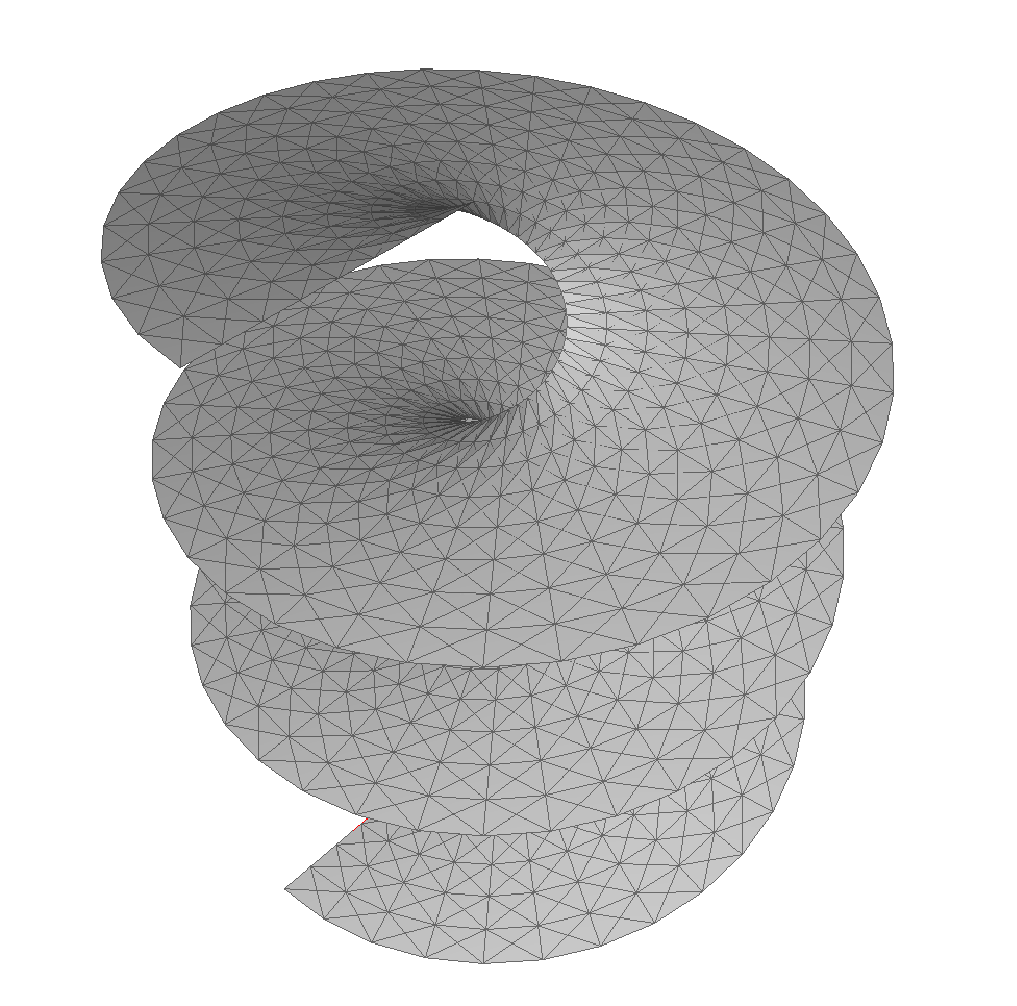
\includegraphics[width=\linewidth,height=\linewidth]{chapter-04/figs/surf-helicoid}%
\end{minipage}
\begin{minipage}[c]{0.38\textwidth}
   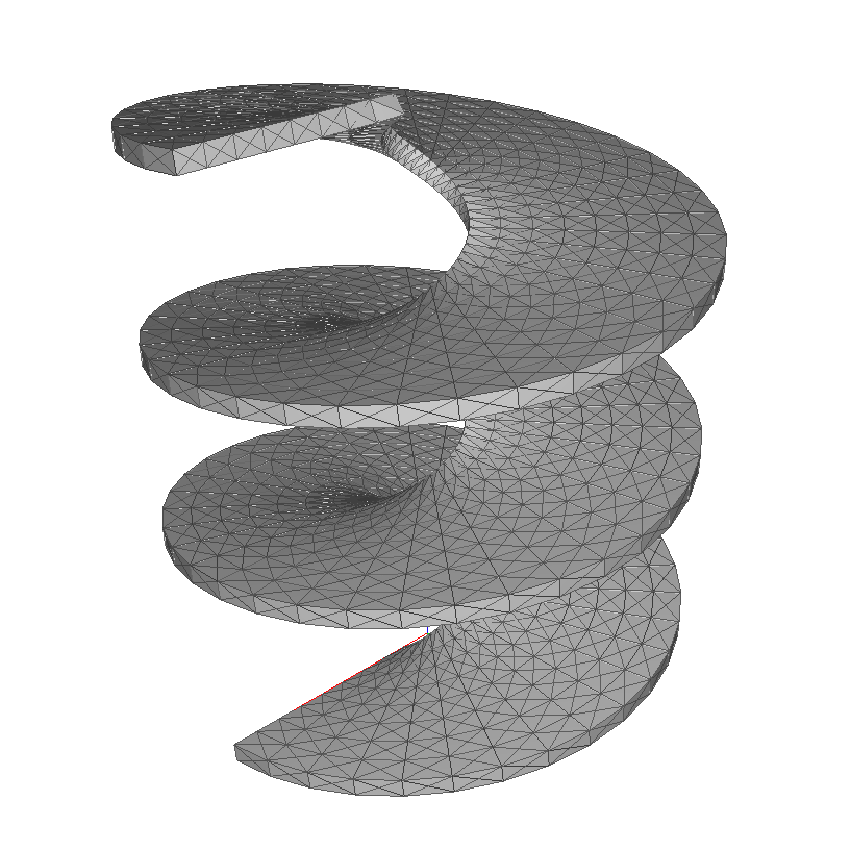
\includegraphics[width=\linewidth,height=\linewidth]{chapter-04/figs/solid-helicoid}%
\end{minipage}%
\caption{Parametrized helicoid values: (a) surface; (b) thin solid.}\label{fig:helicoid}
\end{figure}


\begin{coding}[Turbo pump]\ 
Starting
The main difference with |SOLIDHELICOID| template is the piecewise-linear |Dom2D| mapped from the rectangular |grid2D|.
\begin{lstlisting}[language=JuliaLocal, style=julia, mathescape=true]
function TURBOPUMP(; nturns=3, R=1., r=0.0, shape=[36*nturns,8], pitch=2, thickness=0.1)
   totalangle = nturns*2*pi;  xM = 36*nturns 
   (x0,xm1,xm2,xM) = (0.0, xM/2nturns, 6xM/2nturns, xM)
   G = (x-) x<xm1 ? x/xm1 : (x)xm2 ? 1+(xm2-x)/(xM-xm2) : 1))
   grid2D = INTERVALS(xM)(xM) * INTERVALS(1)(8)
   dom = MAP( p-)begin (u,v)=p; [u, (G(u)+0.1)*v] end )(grid2D)
   Dom2D= T([2])([r])(S([1,2])([totalangle/shape[1],R-r])(dom)) 
   surface = p-)((u,v)=p;[v*cos(u); v*sin(u); u*(pitch/(2*pi))]) 
   solidMapping = THINSOLID(surface)
   Domain3D = Dom2D * INTERVALS(thickness)(1)
   return MAP(solidMapping)(Domain3D)
end
\end{lstlisting}
\end{coding}


\begin{figure}[hbp] %  figure placement: here, top, bottom, or page
   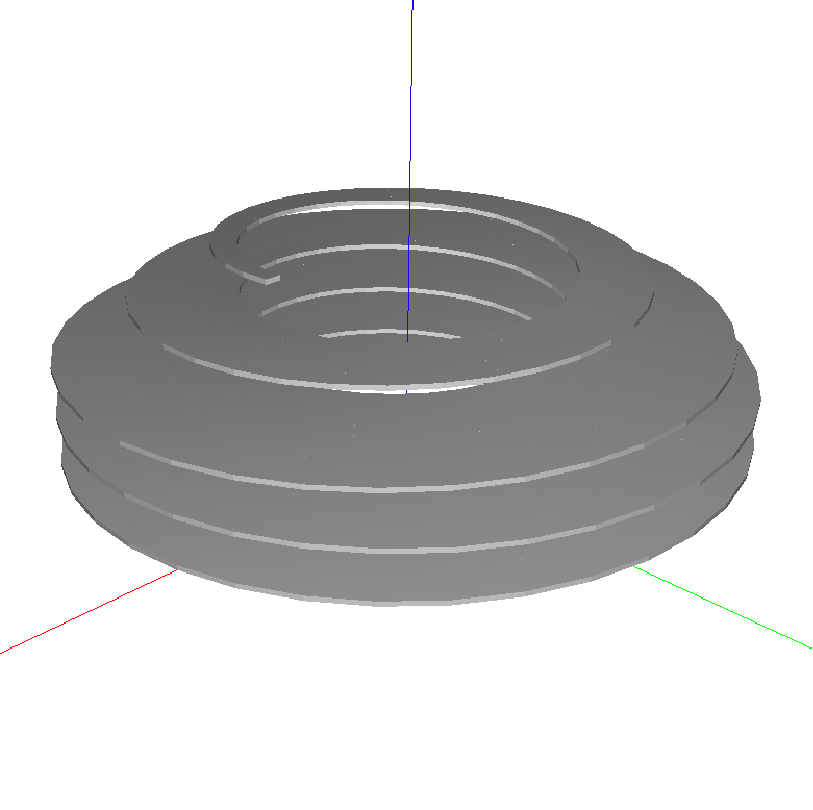
\includegraphics[width=0.337\linewidth]{chapter-04/figs/turbo-pump01}%
   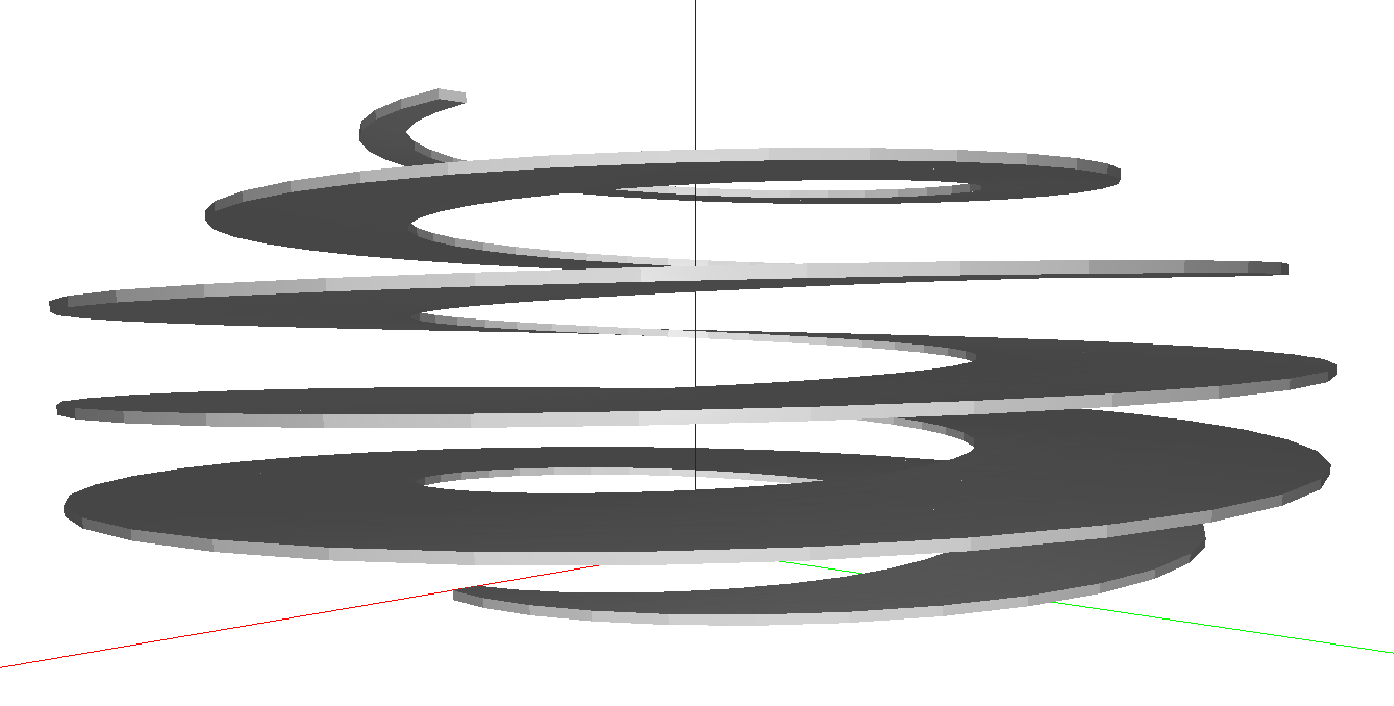
\includegraphics[width=0.663\linewidth]{chapter-04/figs/turbo-pump02}%
\caption{Two prospective images of the turbo pump component: (a) from top; (b) from side.}
\label{fig:turbopump}
\end{figure}

The piecewise linear |dom| shape is produced by the Julia function assigned to symbol |G|, implemented as a nested conditional triple statement. The three subdomain of piecewise |G| domain are defined by |(x0,xm1,xm2,xM)|.

\begin{coding}[Turbo pump’s object viewing]\ 
\begin{lstlisting}[language=JuliaLocal, style=julia, mathescape=true]
obj = TURBOPUMP( pitch=0.15, thickness=0.015, nturns=5, r=1/2 );
view = Dict("background_color"=)[1,1,1]); VIEW(obj, view)
\end{lstlisting}
The other parameters have default value, given in the definition head.
\end{coding}



\section{Attach properties to geometry}\label{sect:4-4}

Any geometric model is usually constituted by its geometry and associated properties or attributes that specify its appearance, like colors, textures, and materials used to render it on the screen or build a concrete instance in the real world. In this section, we shortly discuss some aspects of our interest: (a)~in XML, which was designed to describe the semantics of any kind of data in a computer; (b)  in the IFC standard, oriented to transport building data of architectural, engineering, and construction type between different computer systems. The section concludes with introducing the primitive |PROPERTIES| and |PropertySet| used by our Julia package |Plasm|.

\subsection*{XML Document Object Model (DOM)}\label{sect:4-4-1}

The eXtensible Markup Language (XML) is a software- and hardware-independent tool for storing and transporting data. An XML file is a text-based document that you can save with the |.xml| extension. 

Extensible Markup Language (XML) is a markup language used to describe the content and structure of the data in a document.
At the lemma XML of the Oxford English Dictionary~\cite{}, we find “a metalanguage which allows users to define their \emph{customized} markup languages, especially to display documents on the internet.”

\begin{definition}[Document Type Definition] 
DTD is a Document Type Definition. A DTD defines the structure and the legal \emph{elements} and \emph{attributes} of an XML document.
\end{definition}
XML was designed to carry data, hence with focus on what data are, and is extensible. This means that the author must define both the tags (markup) and the document structure.
The tags used in a document are not defined in any XML standard, but are “invented” by the author of the document.

\begin{definition}[XML Elements] are the basic building block of the XML document. It is used as a container to store text elements, attributes, media objects etc. 
Every XML documents contain at least one element whose scopes are delimited by start and end tags or in case of empty elements it is delimited by an empty tag.
\end{definition}

\begin{definition}[XML Attributes] XML elements can have attributes as sequences of pairs |name|=|”value”| separated by commas. Attributes are designed to contain data related to a specific element. Attribute values must always be quoted.
\end{definition}


\begin{definition}[XML Data Object Model (DOM) documents]
XML DOM documents are modeled using \emph{objects}, and the data model encompasses not only the structure of a document, but also the behavior of the document and the objects of which it is composed. 
\end{definition}

\begin{definition}[Structure Model] The term \emph{structure model} is used to describe the tree-like representation of a document. A tree structure contains a \emph{root} element (as parent), \emph{child} elements, and so on.
\end{definition}

The XML DOM defines also a standard way for accessing and manipulating files that presents an XML document as a tree-structure~\cite{}. 
Everything in such codified documents is a \emph{node}:
the entire document is a document node; every XML element is an element node; the text in the XML elements are text nodes; every attribute is an attribute node; comments are comment nodes. In particular, the DOM is a  language-independent standard API for how to get, change, add, and delete XML nodes.



\subsection*{IFC attributes and properties}\label{sect:4-4-2}

IFC (Industry Foundation Classes) is an Open Data schema and set of formats used to store OpenBIM data.  
The IFC file format and content is discussed in Chapter~\ref{chapt:8}. Some concepts are introduced here for reference and comparison with the definition of |Plasm| function |Properties|.  

\begin{definition}[IFC Entity]
The IFC Entity is a class of information defined by common attributes and constraints. 
It is similar to the term “class” in  programming languages but describing data structure only, not behavior such as methods. 
\end{definition}

All digital data objects in IFC belongs to an IFC class. 
\emph{Attributes} and \emph{properties} are two ways to assign extra metadata to an IFC class. Although they sound similar, they are not the same~\cite{}. 

The |IfcRoot| Entity is unique since it is the root of the information database and provides the four attributes |GlobalId|, |OwnerHistory|, |Name|, |Description|.
IFC classes can be divided into two categories: rooted and non-rooted classes. 
Rooted classes inherit attributes from |IfcRoot| Entity, whereas non-rooted classes do not. 

If a class is a subclass of another class, it inherits the same abilities of that class, such as having specific attributes, properties, or relationships. Subclasses \emph{do not} actually \emph{inherit the values} of the attributes themselves, but only the \emph{ability to have} that attribute. 


\subsubsection*{IFC attributes}\label{sect:4-4-2-1}



Each BIM (Building Information Model) object is assigned to a specific class (Entity), and each class has its attributes. Examples of attributes include Name, Description, PredefinedType, ObjectType, and Tag, where tag (or label) is the identifier at the occurrence level of the particular instance of a product or shape. All IFC classes have attributes. Attributes contain a name, as well as a value.  Attributes may be optional or mandatory. 

\begin{definition}[IFC Attribute]
is an unit of information within an entity, defined by a particular type or reference to a particular entity.
There are three kinds of attributes: \emph{direct}, \emph{inverse}, and \emph{derived} attributes, i.e., scalar values, queries for related data, or computations within the schema, respectively.
\end{definition}

The names of IFC Attributes are fixed, having been defined within the IFC standard. When an IFC class is defined, their attributes must be defined as well, or marked as empty if it is optional. The list of attributes that can be created for each IFC classes is fixed and specified in the IFC specification. 


\subsubsection*{IFC properties}\label{sect:4-4-2-2}

\begin{definition}[IFC Property]
The term “property” is a \emph{unit of information} that is dynamically associated with a particular entity instance, similar to "late-bound" or "run-time" in programming terminology. 
\end{definition}

This definition of “Property” is bound to “occurrence”, “template”, “set of occurrence”, set of “template”, meaning set of property templates serving a common purpose and having applicability to objects of a particular entity.

Unlike attributes, which are defined with each IFC class, properties themselves are an IFC class, and properties themselves have attributes. Also unlike attributes, related properties can be grouped into a |PropertySet|, or Pset, for short. This Pset can exist as its own IFC class, and then be linked to one or more relevant IFC classes. 


\subsection*{Plasm properties}\label{sect:4-4-3}

In |Plasm| we have functions objects and data objects. Every data object of geometric type |obj::Hpc| produced by a geometric |Plasm| function contains a possibly empty field |Properties::Dict{String, Any}| used to allocate a representation of any property, in particular of \emph{appearance} ones.  

Each |Hpc| value is a DAG (directed acyclic graph) node, root of the subtree whose children are mapped from the field |childs::Array|. The values of properties extend to the whole rooted subgraph, unless redefined locally.

The |childs| of a |Hpc| node may be either of |Hpc| or |Geometry| type. The |Geometry| node may have any subset of non-empty elements from:
\begin{lstlisting}[language=JuliaLocal, style=julia, mathescape=true]
points::Vector{Vector{Float64}}
edges::Vector{Vector{Int}}
faces::Vector{Vector{Int}}
hulls::Vector{Vector{Int}}
\end{lstlisting}
corresponding to 0-, 1-, 2-, and 3-dimensional (convex) cells, respectively. 

The |Plasm| type |Lar| is a flat version of |Hpc|+|Geometry|, allowing to make algebraic topological computations relative to the search of 3D atoms, that are B-reps of the basis  3-chain allowing to compute any symbolic form of the Boolean algebra induced by a collection of solid primitives (see Chapter~\ref{chapt:4}). 

Of course, there is no isomorphism between the two maps |Hpc|$\to$|Lar| and |Lar|$\to$|Hpc|.  In other words, their composition is not the identity map.

The standard properties of a value |obj::Lar| are the incidence relations between its cells, in either |Vector{Vector}| or in |SparseMatrix| form. In both case they can be extracted as |Dict| values associated to Julia’s symbol keys.


The predefined |Plasm| |PropertySet| are mostly related to graphics appearance, and in particular to the |mutable struct GLBatch|, used  by the module |Plasm/Viewer.jl| to send well-formed packets of graphical information to the GPU for rendering.

\begin{definition}[Appearance \sf PropertySet]
Currently, we have four classes of |PropertySet| to use (1) with general |Hpc| values (default); (2) with {\sf Viewer} objects (viewing); (3) when “exploding” assemplies of |Hpc|s (explode); (4) when showing a cellular complex annotated with cells indices (number).
\end{definition}

\begin{lstlisting}[language=JuliaLocal, style=julia, mathescape=true]
typeof(PROPERTIES)
# typeof(PROPERTIES) (singleton type of function PROPERTIES, subtype of Function)

function PSET()  <: PROPERTIES end;
function PVIEW() <: PROPERTIES end;
function PEXPL() <: PROPERTIES end;
function PNUM()  <: PROPERTIES end;

function PropertySet() <: Union{PSET, PVIEW, PEXPL, PNUM} end 
# PropertySet (generic function with 1 method)
\end{lstlisting}

\subsubsection*{\small\sf PSET <: PROPERTIES}\label{4-4-3-1}

|PSET| is the default |PropertySet| associated to the appearance of any geometric value, either isolated or aggregated within a single root of |Hpc| type. 


\subsubsection*{\small\sf PVIEW <: PROPERTIES}\label{4-4-3-2}

|PVIEW| associates the default |PropertySet| to the interaction session, i.e., to the ability to handle joystick, keyboard, and mouse within a visualizer window containing an OpenGL context made available by the |ModernGL| package.


\subsubsection*{\small\sf PEXPL <: PROPERTIES}\label{4-4-3-3}

In order to manage a parametric explosion of a geometric object, defined as aggregation of simpler objects through a |STRUCT| primitive, we setup the |PEXPL| independent scaling parameters $s_x, s_y, s_z$ of each shape component’s centroid, either as 3-,  2-, and 1-cell complex. 



\subsubsection*{\small\sf PNUM <: PROPERTIES}\label{4-4-3-4}

Similarly to the previous case, the 
|PNUM| default |PropertySet| is used for the visualization of cells’ indices in  interaction sessions with a complicated geometric value, i.e., when looking at the text oindices of cells. It must specify a number of predefined properties concerning the size of text characters with respect to the bounding box size of current content of the viewing volume, as well as the colors and sizes of the different subsets of $d$-cells. 
The cell numbering is used for check and debug of geometric values. 


\section{Design documentation notebooks}\label{sect:4-5}

A virtual notebook environment is used for literate programming~\cite{10.1093.27.2.97}, a method of writing computer programs together with explanations and documentation, mostly using |Markdown| rich text~\footnote{Useful reference:\href{https://www.markdownguide.org/basic-syntax/}{https://www.markdownguide.org/basic-syntax/}.} in the last two decades. “Literate programming is a methodology that combines a programming language with a documentation language, thereby making programs more robust, more portable, more easily maintained, and arguably more fun to write than programs that are written only in a high-level language.”~\cite{Knuth:92}


A notebook is a computer document, specifically a file shareable with internet protocols, that merges source code, plain descriptions, data, and visualizations like function graphs and 3D models. It provides fast, shareable objects (files), to be used through an interactive environment, and useful for prototyping code, exploring and visualizing data, and sharing ideas with others.




\begin{figure}[htbp] %  figure placement: here, top, bottom, or page
   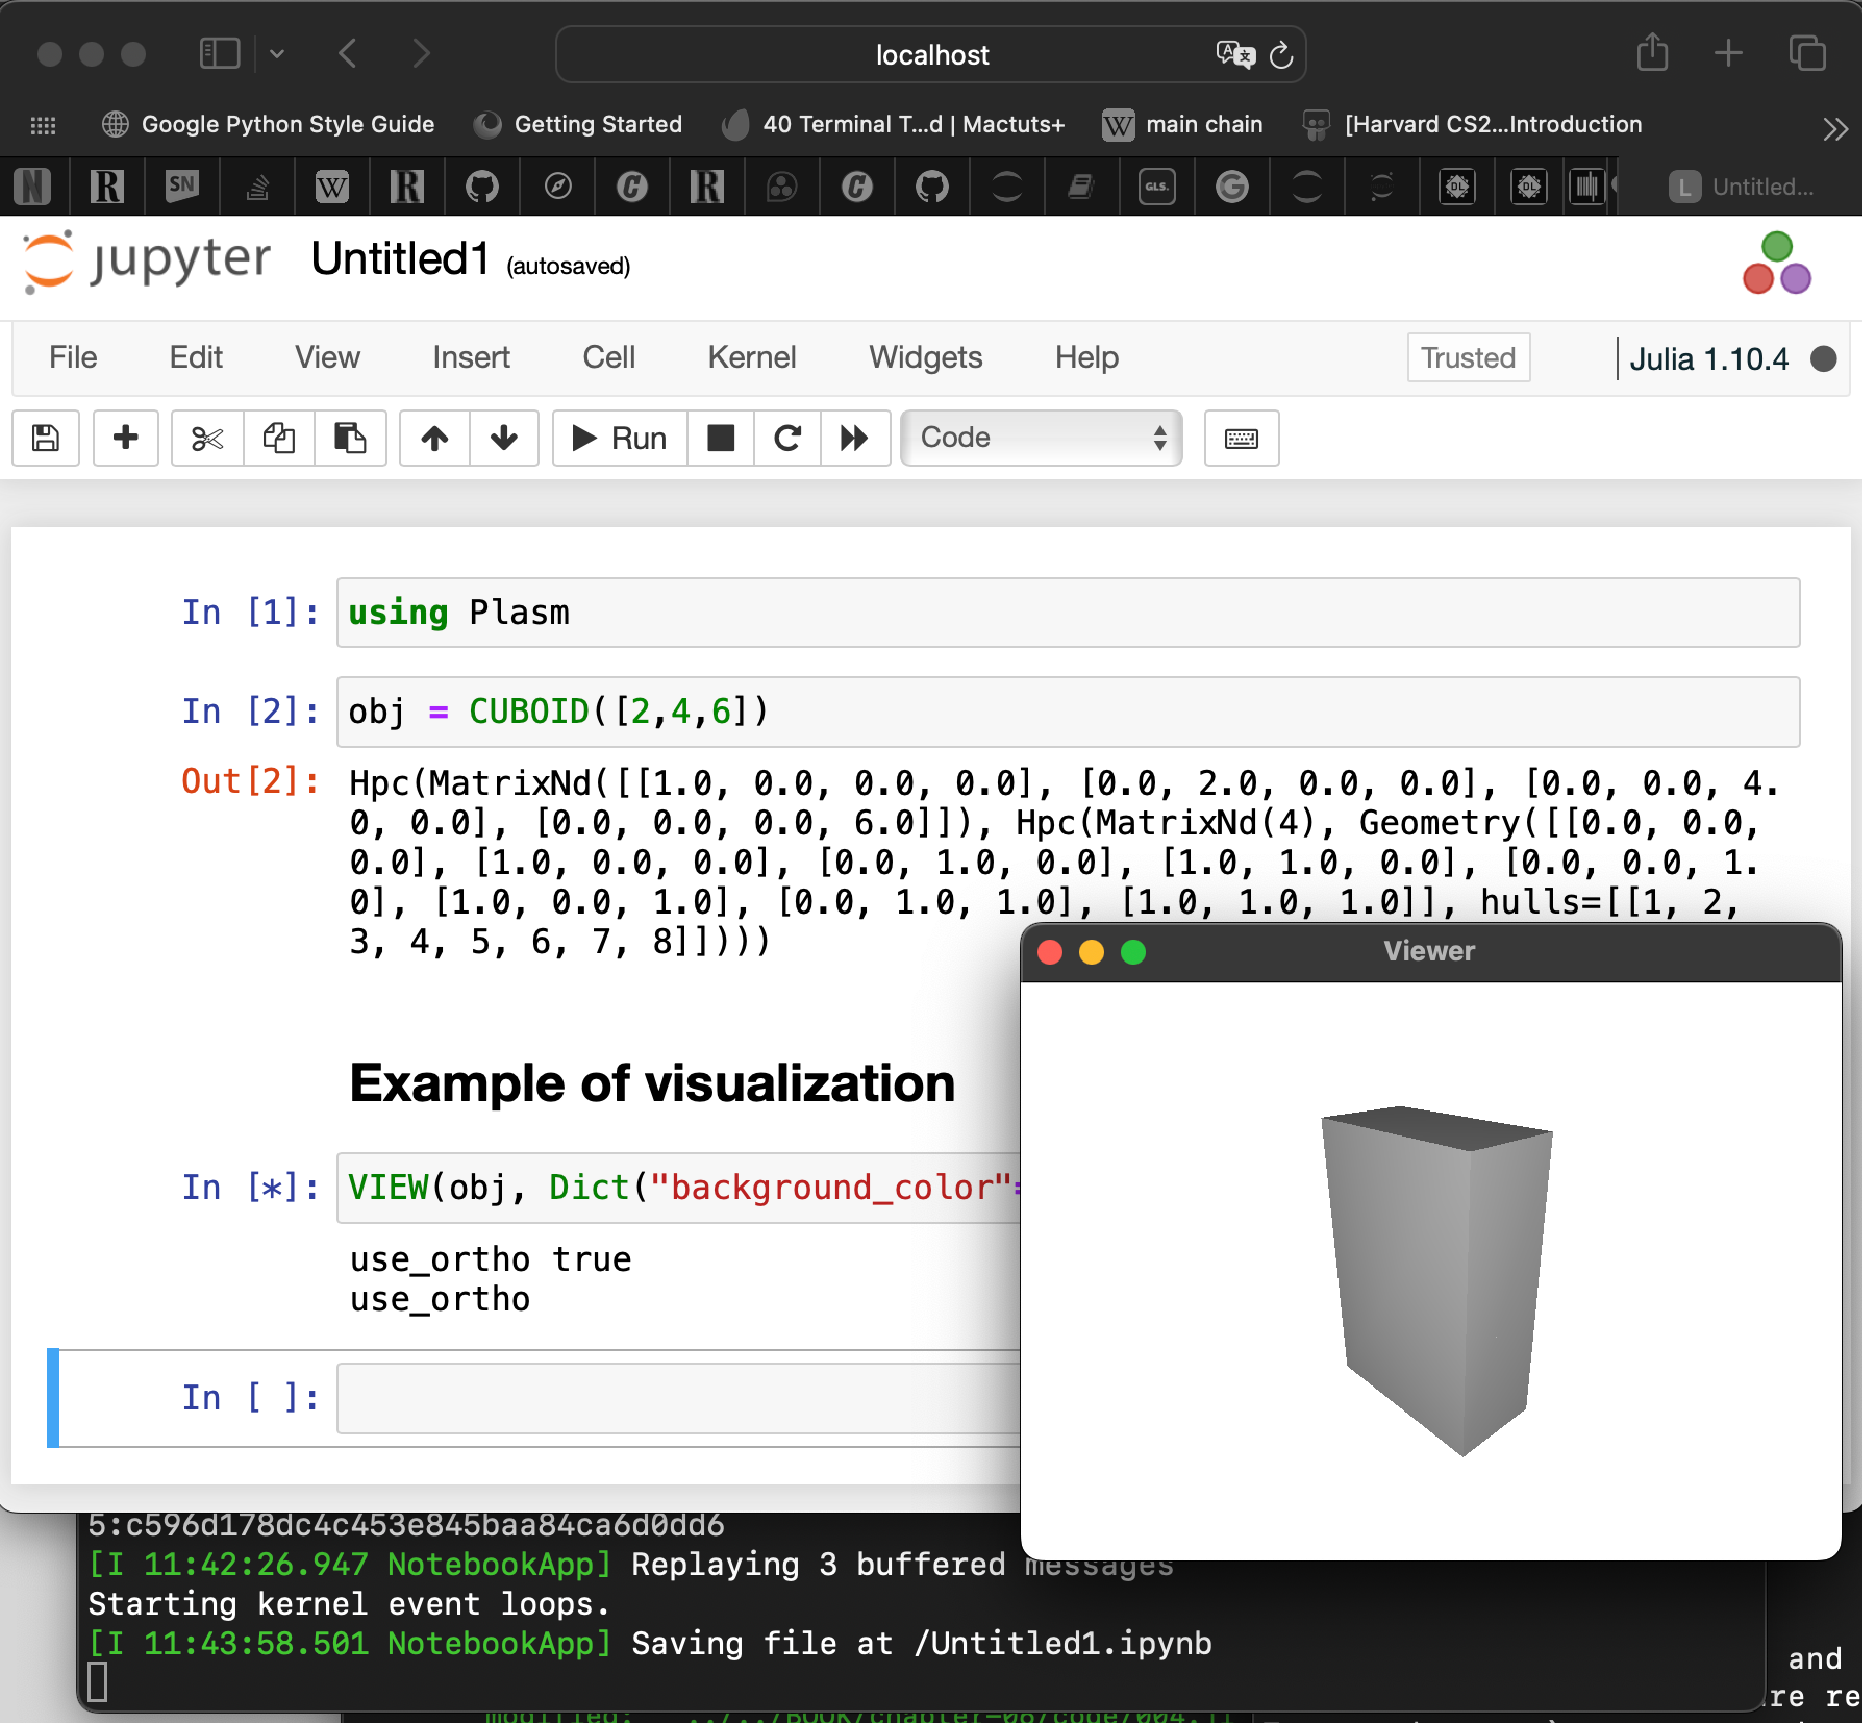
\includegraphics[width=\linewidth]{chapter-04/figs/jupyter}%
\caption{A small test session in Julia Jupiter using Plasm.}
\label{fig:jupyter}
\end{figure}


\subsubsection*{Install Julia notebook}\label{sect:4-5-1}


The Jupyter platform is a web-based interactive computing software. 
A Jupyter notebook is a web document (text file) with |.ipynb| sufffix.
The notebook combines live code, equations, narrative text, and 3D visualizations. It lets you run source code piece by piece, which is helpful when you're just imagining things and testing the ideas to develop with computer code, making it easier to understand what you're doing.
Project Jupyter's name refers to the three core programming languages supported by Jupyter: Julia, Python, and R. Currently, the Jupyter system supports over 100 programming languages, called "kernels" in the Jupyter ecosystem.

Julia Jupiter notebooks are very easy to install. 
Just write (the first time) to your Julia |REPL| console. 

\begin{lstlisting}[language=JuliaLocal, style=julia, mathescape=true]
julia> ]add IJulia 
\end{lstlisting}

When the package is installed, with |<backspace>| you will return to the standard |julia>| interactive mode.  Now write:

\begin{lstlisting}[language=JuliaLocal, style=julia, mathescape=true]
julia> using IJulia   

julia> notebook()
\end{lstlisting}
and wait few seconds. |Julia| will launch in background a |Jupyter| server and open a page on jour default web browser, asking to navigate the disk and either open a new file to work or one already existent and previously saved.


\subsubsection*{Install Julia Plasm package}\label{sect:4-5-1}

It is even more easier than the above; see Figure~\ref{fig:jupyter}. Of course, the output cell does not exists when the last line of code  terminates with a semicolon punctuation mark.

The reader should pay attention to some facts: (a) this notebook is a web document named |Untitled1.ipynb| and served locally from the machine’s |localhost|; (b) the language kernel (look top-right) is |Julia 1.10.4|; (c) the small circle close to it is black since the kernel has not already released control since the 3D window viewer is interactive; (d) it must be closed to go ahead; (e) the page is made by numbered |In| and |Out| cells, four of type |Code| and one of type |Markdown|; (f) an asterisk is on the right of the currently working cells.

\section{Export geometry}\label{sect:4-6}

There are several ways to export either produced or in-progress geometric |Plasm| models, starting from directly exporting the Julia sources. Depending on the size of the building project, the digital project evaluated within a short number of seconds of computing time could easily amount to datasets many hundreds of thousands of times more significant. 

Of course, the |Plasm| platform may also export/import Computer Graphics standard formats for polyhedral modeling, particularly using the boundary representation of the Boolean algebras’ atoms associated with the building design. The simplest options for file transport of geometry are boundary triangulations or polygons, directly representable through the |PolygonSet| entity primitives of the IFC file standard.

\subsubsection*{Direct export/import of sources}\label{sect:4-6-1}

Julia has two mechanisms for loading source code: \emph{code inclusion} and \emph{package loading}~\cite{}.
Code inclusion is relatively straightforward: it evaluates the given source file in the context of the caller process. It is good practice when writing a source file scheduled to export a geometric model (1) to choose a possibly long but semantically significant name and (2) to conclude each such file with one or more model |VIEW()|s of the exported building parts/aggregates. Inclusion also allows you to split a single program across multiple source files.

The expression |include("source.jl")| causes the contents of the file |"source.jl"| to be evaluated in the global scope of the module where the include call occurs. The expression |include()| can be called multiple times with the same file, and the file is evaluated every time. 

The second mechanism, \emph{package loading}, is more general and powerful. The |import <name>| or |using <name>| allows you to load a package—i.e., an independent, reusable collection of Julia code, wrapped in one or more module, and makes the resulting software library available by the name |<name>| inside the importing module~\cite{}. 

\begin{remark}
Creating a specialized Julia module or package for a specific architectural or engineering  project may be of great professional interest and economic satisfaction. 
E.g., the project could import Julia packages for the building typology under consideration, if any. In architecture, typology refers to identifying and grouping buildings according to their kind of use and similarity of essential characteristics, such as Residential, Educational, Institutional, Commercial, Business, or Industrial Buildings.
\end{remark}

\begin{remark}
You can have subtypes in each type with characteristic morphology: for example, in residential higher education, or in various types of specialty hospital establishment, which must follow strict legal requirements, and so on.
In addition, the specific design package might import parametric |Plasm| functions already developed for similar constructions and enrich them with new function methods finalized to the singular, unique design structure and shape under development.
\end{remark}

This kind of digital innovation process, on top of BIM and IFC standards (see Chapter~\ref{chapt:10}), could be of significant interest in case of development programs launched as sectorial construction interventions by governments (say housing, schools, etc.) or by charitable foundations in developing countries, where some standardization can greatly reduce the program costs.
 

\subsubsection*{Unevaluated/Evaluated/Binary LAR format}\label{sect:4-6-2}

Linear Algebraic Representation (|LAR|) is the name of the algebraic geometrical data structures and computational pipeline developed by the authors and others in the last decade, and embedded recently in |Plasm|. This data structure has various formats, depending on the advancement of computation. In particular, three LAR states may be expressed as unevaluated, evaluated, and binary.

\begin{description} 
\item[Unevaluated LAR] Sparse binary matrices that encode the cells of a cellular complex as incidence relations between $d$-cellls and $0$-cells ($0 \leq d \leq 3$). All the binary relations between cells of different dimensions can be easily generated. The occupied storage space is less or equal to that of common incidence structures in graphics and solid modeling.

\item[Evaluated LAR] is a pair (\emph{geometry}, \emph{topology}) where \emph{geometry} is the matrix |V::Matrix{Float64{| of coordinates of 0-cells (|V::Matrix{Float64}|), and \emph{topology} is a triple (in 3D) of sparse binary matrices, encoding the coboundary operators $\delta_0, \delta_1, \delta_2$ corresponding to incidence relations |VE|, |EF|, and |FC|. These result by the 3D algorithmic \emph{arrangement} pipeline that partitions the Euclidean 3-space on the boundary surfaces of any given collection of |Brep| solid models.

\item[Binary LAR] is the result of computation of the binary algebra induced by the spatial collocation and orientation of the whole collection of B-rep primitives and solids considered by the designer at the beginning of the computational pipeline, i.e., when all the geometric elements were collocated within the geometric design of the considered building portion. This binary matrix has number of columns equal to the number of computed atoms of the space arrangement and number of rows equal to the number of primitive shapes (of uniform material) used in a geometric design.
\end{description}

Every noteworthy subset of design atoms, selected by any reason---in particular, to assign material properties, catalog products, or compute volumes or cost---will be  extracted as a subset of corresponding columns and rows.

\subsubsection*{IFC PolygonSet file format}\label{sect:4-6-3}

Our preliminary tests showed that all the |Plasm| geometric shapes we defined or selected are exportable to transport file |IFC| as |PolygonSet| entities and their associated entities concerning polygons or triangles, vertex indices, and vertex coordinates. This point will be treated extensively in Chapter~\ref{chapt:10}.


